\documentclass{article}
\usepackage{iclr2027_conference,times}
%%%%% NEW MATH DEFINITIONS %%%%%

\usepackage{amsmath,amsfonts,bm}

% Mark sections of captions for referring to divisions of figures
\newcommand{\figleft}{{\em (Left)}}
\newcommand{\figcenter}{{\em (Center)}}
\newcommand{\figright}{{\em (Right)}}
\newcommand{\figtop}{{\em (Top)}}
\newcommand{\figbottom}{{\em (Bottom)}}
\newcommand{\captiona}{{\em (a)}}
\newcommand{\captionb}{{\em (b)}}
\newcommand{\captionc}{{\em (c)}}
\newcommand{\captiond}{{\em (d)}}

% Highlight a newly defined term
\newcommand{\newterm}[1]{{\bf #1}}


% Figure reference, lower-case.
\def\figref#1{figure~\ref{#1}}
% Figure reference, capital. For start of sentence
\def\Figref#1{Figure~\ref{#1}}
\def\twofigref#1#2{figures \ref{#1} and \ref{#2}}
\def\quadfigref#1#2#3#4{figures \ref{#1}, \ref{#2}, \ref{#3} and \ref{#4}}
% Section reference, lower-case.
\def\secref#1{section~\ref{#1}}
% Section reference, capital.
\def\Secref#1{Section~\ref{#1}}
% Reference to two sections.
\def\twosecrefs#1#2{sections \ref{#1} and \ref{#2}}
% Reference to three sections.
\def\secrefs#1#2#3{sections \ref{#1}, \ref{#2} and \ref{#3}}
% Reference to an equation, lower-case.
\def\eqref#1{equation~\ref{#1}}
% Reference to an equation, upper case
\def\Eqref#1{Equation~\ref{#1}}
% A raw reference to an equation---avoid using if possible
\def\plaineqref#1{\ref{#1}}
% Reference to a chapter, lower-case.
\def\chapref#1{chapter~\ref{#1}}
% Reference to an equation, upper case.
\def\Chapref#1{Chapter~\ref{#1}}
% Reference to a range of chapters
\def\rangechapref#1#2{chapters\ref{#1}--\ref{#2}}
% Reference to an algorithm, lower-case.
\def\algref#1{algorithm~\ref{#1}}
% Reference to an algorithm, upper case.
\def\Algref#1{Algorithm~\ref{#1}}
\def\twoalgref#1#2{algorithms \ref{#1} and \ref{#2}}
\def\Twoalgref#1#2{Algorithms \ref{#1} and \ref{#2}}
% Reference to a part, lower case
\def\partref#1{part~\ref{#1}}
% Reference to a part, upper case
\def\Partref#1{Part~\ref{#1}}
\def\twopartref#1#2{parts \ref{#1} and \ref{#2}}

\def\ceil#1{\lceil #1 \rceil}
\def\floor#1{\lfloor #1 \rfloor}
\def\1{\bm{1}}
\newcommand{\train}{\mathcal{D}}
\newcommand{\valid}{\mathcal{D_{\mathrm{valid}}}}
\newcommand{\test}{\mathcal{D_{\mathrm{test}}}}

\def\eps{{\epsilon}}


% Random variables
\def\reta{{\textnormal{$\eta$}}}
\def\ra{{\textnormal{a}}}
\def\rb{{\textnormal{b}}}
\def\rc{{\textnormal{c}}}
\def\rd{{\textnormal{d}}}
\def\re{{\textnormal{e}}}
\def\rf{{\textnormal{f}}}
\def\rg{{\textnormal{g}}}
\def\rh{{\textnormal{h}}}
\def\ri{{\textnormal{i}}}
\def\rj{{\textnormal{j}}}
\def\rk{{\textnormal{k}}}
\def\rl{{\textnormal{l}}}
% rm is already a command, just don't name any random variables m
\def\rn{{\textnormal{n}}}
\def\ro{{\textnormal{o}}}
\def\rp{{\textnormal{p}}}
\def\rq{{\textnormal{q}}}
\def\rr{{\textnormal{r}}}
\def\rs{{\textnormal{s}}}
\def\rt{{\textnormal{t}}}
\def\ru{{\textnormal{u}}}
\def\rv{{\textnormal{v}}}
\def\rw{{\textnormal{w}}}
\def\rx{{\textnormal{x}}}
\def\ry{{\textnormal{y}}}
\def\rz{{\textnormal{z}}}

% Random vectors
\def\rvepsilon{{\mathbf{\epsilon}}}
\def\rvtheta{{\mathbf{\theta}}}
\def\rva{{\mathbf{a}}}
\def\rvb{{\mathbf{b}}}
\def\rvc{{\mathbf{c}}}
\def\rvd{{\mathbf{d}}}
\def\rve{{\mathbf{e}}}
\def\rvf{{\mathbf{f}}}
\def\rvg{{\mathbf{g}}}
\def\rvh{{\mathbf{h}}}
\def\rvu{{\mathbf{i}}}
\def\rvj{{\mathbf{j}}}
\def\rvk{{\mathbf{k}}}
\def\rvl{{\mathbf{l}}}
\def\rvm{{\mathbf{m}}}
\def\rvn{{\mathbf{n}}}
\def\rvo{{\mathbf{o}}}
\def\rvp{{\mathbf{p}}}
\def\rvq{{\mathbf{q}}}
\def\rvr{{\mathbf{r}}}
\def\rvs{{\mathbf{s}}}
\def\rvt{{\mathbf{t}}}
\def\rvu{{\mathbf{u}}}
\def\rvv{{\mathbf{v}}}
\def\rvw{{\mathbf{w}}}
\def\rvx{{\mathbf{x}}}
\def\rvy{{\mathbf{y}}}
\def\rvz{{\mathbf{z}}}

% Elements of random vectors
\def\erva{{\textnormal{a}}}
\def\ervb{{\textnormal{b}}}
\def\ervc{{\textnormal{c}}}
\def\ervd{{\textnormal{d}}}
\def\erve{{\textnormal{e}}}
\def\ervf{{\textnormal{f}}}
\def\ervg{{\textnormal{g}}}
\def\ervh{{\textnormal{h}}}
\def\ervi{{\textnormal{i}}}
\def\ervj{{\textnormal{j}}}
\def\ervk{{\textnormal{k}}}
\def\ervl{{\textnormal{l}}}
\def\ervm{{\textnormal{m}}}
\def\ervn{{\textnormal{n}}}
\def\ervo{{\textnormal{o}}}
\def\ervp{{\textnormal{p}}}
\def\ervq{{\textnormal{q}}}
\def\ervr{{\textnormal{r}}}
\def\ervs{{\textnormal{s}}}
\def\ervt{{\textnormal{t}}}
\def\ervu{{\textnormal{u}}}
\def\ervv{{\textnormal{v}}}
\def\ervw{{\textnormal{w}}}
\def\ervx{{\textnormal{x}}}
\def\ervy{{\textnormal{y}}}
\def\ervz{{\textnormal{z}}}

% Random matrices
\def\rmA{{\mathbf{A}}}
\def\rmB{{\mathbf{B}}}
\def\rmC{{\mathbf{C}}}
\def\rmD{{\mathbf{D}}}
\def\rmE{{\mathbf{E}}}
\def\rmF{{\mathbf{F}}}
\def\rmG{{\mathbf{G}}}
\def\rmH{{\mathbf{H}}}
\def\rmI{{\mathbf{I}}}
\def\rmJ{{\mathbf{J}}}
\def\rmK{{\mathbf{K}}}
\def\rmL{{\mathbf{L}}}
\def\rmM{{\mathbf{M}}}
\def\rmN{{\mathbf{N}}}
\def\rmO{{\mathbf{O}}}
\def\rmP{{\mathbf{P}}}
\def\rmQ{{\mathbf{Q}}}
\def\rmR{{\mathbf{R}}}
\def\rmS{{\mathbf{S}}}
\def\rmT{{\mathbf{T}}}
\def\rmU{{\mathbf{U}}}
\def\rmV{{\mathbf{V}}}
\def\rmW{{\mathbf{W}}}
\def\rmX{{\mathbf{X}}}
\def\rmY{{\mathbf{Y}}}
\def\rmZ{{\mathbf{Z}}}

% Elements of random matrices
\def\ermA{{\textnormal{A}}}
\def\ermB{{\textnormal{B}}}
\def\ermC{{\textnormal{C}}}
\def\ermD{{\textnormal{D}}}
\def\ermE{{\textnormal{E}}}
\def\ermF{{\textnormal{F}}}
\def\ermG{{\textnormal{G}}}
\def\ermH{{\textnormal{H}}}
\def\ermI{{\textnormal{I}}}
\def\ermJ{{\textnormal{J}}}
\def\ermK{{\textnormal{K}}}
\def\ermL{{\textnormal{L}}}
\def\ermM{{\textnormal{M}}}
\def\ermN{{\textnormal{N}}}
\def\ermO{{\textnormal{O}}}
\def\ermP{{\textnormal{P}}}
\def\ermQ{{\textnormal{Q}}}
\def\ermR{{\textnormal{R}}}
\def\ermS{{\textnormal{S}}}
\def\ermT{{\textnormal{T}}}
\def\ermU{{\textnormal{U}}}
\def\ermV{{\textnormal{V}}}
\def\ermW{{\textnormal{W}}}
\def\ermX{{\textnormal{X}}}
\def\ermY{{\textnormal{Y}}}
\def\ermZ{{\textnormal{Z}}}

% Vectors
\def\vzero{{\bm{0}}}
\def\vone{{\bm{1}}}
\def\vmu{{\bm{\mu}}}
\def\vtheta{{\bm{\theta}}}
\def\va{{\bm{a}}}
\def\vb{{\bm{b}}}
\def\vc{{\bm{c}}}
\def\vd{{\bm{d}}}
\def\ve{{\bm{e}}}
\def\vf{{\bm{f}}}
\def\vg{{\bm{g}}}
\def\vh{{\bm{h}}}
\def\vi{{\bm{i}}}
\def\vj{{\bm{j}}}
\def\vk{{\bm{k}}}
\def\vl{{\bm{l}}}
\def\vm{{\bm{m}}}
\def\vn{{\bm{n}}}
\def\vo{{\bm{o}}}
\def\vp{{\bm{p}}}
\def\vq{{\bm{q}}}
\def\vr{{\bm{r}}}
\def\vs{{\bm{s}}}
\def\vt{{\bm{t}}}
\def\vu{{\bm{u}}}
\def\vv{{\bm{v}}}
\def\vw{{\bm{w}}}
\def\vx{{\bm{x}}}
\def\vy{{\bm{y}}}
\def\vz{{\bm{z}}}

% Elements of vectors
\def\evalpha{{\alpha}}
\def\evbeta{{\beta}}
\def\evepsilon{{\epsilon}}
\def\evlambda{{\lambda}}
\def\evomega{{\omega}}
\def\evmu{{\mu}}
\def\evpsi{{\psi}}
\def\evsigma{{\sigma}}
\def\evtheta{{\theta}}
\def\eva{{a}}
\def\evb{{b}}
\def\evc{{c}}
\def\evd{{d}}
\def\eve{{e}}
\def\evf{{f}}
\def\evg{{g}}
\def\evh{{h}}
\def\evi{{i}}
\def\evj{{j}}
\def\evk{{k}}
\def\evl{{l}}
\def\evm{{m}}
\def\evn{{n}}
\def\evo{{o}}
\def\evp{{p}}
\def\evq{{q}}
\def\evr{{r}}
\def\evs{{s}}
\def\evt{{t}}
\def\evu{{u}}
\def\evv{{v}}
\def\evw{{w}}
\def\evx{{x}}
\def\evy{{y}}
\def\evz{{z}}

% Matrix
\def\mA{{\bm{A}}}
\def\mB{{\bm{B}}}
\def\mC{{\bm{C}}}
\def\mD{{\bm{D}}}
\def\mE{{\bm{E}}}
\def\mF{{\bm{F}}}
\def\mG{{\bm{G}}}
\def\mH{{\bm{H}}}
\def\mI{{\bm{I}}}
\def\mJ{{\bm{J}}}
\def\mK{{\bm{K}}}
\def\mL{{\bm{L}}}
\def\mM{{\bm{M}}}
\def\mN{{\bm{N}}}
\def\mO{{\bm{O}}}
\def\mP{{\bm{P}}}
\def\mQ{{\bm{Q}}}
\def\mR{{\bm{R}}}
\def\mS{{\bm{S}}}
\def\mT{{\bm{T}}}
\def\mU{{\bm{U}}}
\def\mV{{\bm{V}}}
\def\mW{{\bm{W}}}
\def\mX{{\bm{X}}}
\def\mY{{\bm{Y}}}
\def\mZ{{\bm{Z}}}
\def\mBeta{{\bm{\beta}}}
\def\mPhi{{\bm{\Phi}}}
\def\mLambda{{\bm{\Lambda}}}
\def\mSigma{{\bm{\Sigma}}}

% Tensor
\DeclareMathAlphabet{\mathsfit}{\encodingdefault}{\sfdefault}{m}{sl}
\SetMathAlphabet{\mathsfit}{bold}{\encodingdefault}{\sfdefault}{bx}{n}
\newcommand{\tens}[1]{\bm{\mathsfit{#1}}}
\def\tA{{\tens{A}}}
\def\tB{{\tens{B}}}
\def\tC{{\tens{C}}}
\def\tD{{\tens{D}}}
\def\tE{{\tens{E}}}
\def\tF{{\tens{F}}}
\def\tG{{\tens{G}}}
\def\tH{{\tens{H}}}
\def\tI{{\tens{I}}}
\def\tJ{{\tens{J}}}
\def\tK{{\tens{K}}}
\def\tL{{\tens{L}}}
\def\tM{{\tens{M}}}
\def\tN{{\tens{N}}}
\def\tO{{\tens{O}}}
\def\tP{{\tens{P}}}
\def\tQ{{\tens{Q}}}
\def\tR{{\tens{R}}}
\def\tS{{\tens{S}}}
\def\tT{{\tens{T}}}
\def\tU{{\tens{U}}}
\def\tV{{\tens{V}}}
\def\tW{{\tens{W}}}
\def\tX{{\tens{X}}}
\def\tY{{\tens{Y}}}
\def\tZ{{\tens{Z}}}


% Graph
\def\gA{{\mathcal{A}}}
\def\gB{{\mathcal{B}}}
\def\gC{{\mathcal{C}}}
\def\gD{{\mathcal{D}}}
\def\gE{{\mathcal{E}}}
\def\gF{{\mathcal{F}}}
\def\gG{{\mathcal{G}}}
\def\gH{{\mathcal{H}}}
\def\gI{{\mathcal{I}}}
\def\gJ{{\mathcal{J}}}
\def\gK{{\mathcal{K}}}
\def\gL{{\mathcal{L}}}
\def\gM{{\mathcal{M}}}
\def\gN{{\mathcal{N}}}
\def\gO{{\mathcal{O}}}
\def\gP{{\mathcal{P}}}
\def\gQ{{\mathcal{Q}}}
\def\gR{{\mathcal{R}}}
\def\gS{{\mathcal{S}}}
\def\gT{{\mathcal{T}}}
\def\gU{{\mathcal{U}}}
\def\gV{{\mathcal{V}}}
\def\gW{{\mathcal{W}}}
\def\gX{{\mathcal{X}}}
\def\gY{{\mathcal{Y}}}
\def\gZ{{\mathcal{Z}}}

% Sets
\def\sA{{\mathbb{A}}}
\def\sB{{\mathbb{B}}}
\def\sC{{\mathbb{C}}}
\def\sD{{\mathbb{D}}}
% Don't use a set called E, because this would be the same as our symbol
% for expectation.
\def\sF{{\mathbb{F}}}
\def\sG{{\mathbb{G}}}
\def\sH{{\mathbb{H}}}
\def\sI{{\mathbb{I}}}
\def\sJ{{\mathbb{J}}}
\def\sK{{\mathbb{K}}}
\def\sL{{\mathbb{L}}}
\def\sM{{\mathbb{M}}}
\def\sN{{\mathbb{N}}}
\def\sO{{\mathbb{O}}}
\def\sP{{\mathbb{P}}}
\def\sQ{{\mathbb{Q}}}
\def\sR{{\mathbb{R}}}
\def\sS{{\mathbb{S}}}
\def\sT{{\mathbb{T}}}
\def\sU{{\mathbb{U}}}
\def\sV{{\mathbb{V}}}
\def\sW{{\mathbb{W}}}
\def\sX{{\mathbb{X}}}
\def\sY{{\mathbb{Y}}}
\def\sZ{{\mathbb{Z}}}

% Entries of a matrix
\def\emLambda{{\Lambda}}
\def\emA{{A}}
\def\emB{{B}}
\def\emC{{C}}
\def\emD{{D}}
\def\emE{{E}}
\def\emF{{F}}
\def\emG{{G}}
\def\emH{{H}}
\def\emI{{I}}
\def\emJ{{J}}
\def\emK{{K}}
\def\emL{{L}}
\def\emM{{M}}
\def\emN{{N}}
\def\emO{{O}}
\def\emP{{P}}
\def\emQ{{Q}}
\def\emR{{R}}
\def\emS{{S}}
\def\emT{{T}}
\def\emU{{U}}
\def\emV{{V}}
\def\emW{{W}}
\def\emX{{X}}
\def\emY{{Y}}
\def\emZ{{Z}}
\def\emSigma{{\Sigma}}

% entries of a tensor
% Same font as tensor, without \bm wrapper
\newcommand{\etens}[1]{\mathsfit{#1}}
\def\etLambda{{\etens{\Lambda}}}
\def\etA{{\etens{A}}}
\def\etB{{\etens{B}}}
\def\etC{{\etens{C}}}
\def\etD{{\etens{D}}}
\def\etE{{\etens{E}}}
\def\etF{{\etens{F}}}
\def\etG{{\etens{G}}}
\def\etH{{\etens{H}}}
\def\etI{{\etens{I}}}
\def\etJ{{\etens{J}}}
\def\etK{{\etens{K}}}
\def\etL{{\etens{L}}}
\def\etM{{\etens{M}}}
\def\etN{{\etens{N}}}
\def\etO{{\etens{O}}}
\def\etP{{\etens{P}}}
\def\etQ{{\etens{Q}}}
\def\etR{{\etens{R}}}
\def\etS{{\etens{S}}}
\def\etT{{\etens{T}}}
\def\etU{{\etens{U}}}
\def\etV{{\etens{V}}}
\def\etW{{\etens{W}}}
\def\etX{{\etens{X}}}
\def\etY{{\etens{Y}}}
\def\etZ{{\etens{Z}}}

% The true underlying data generating distribution
\newcommand{\pdata}{p_{\rm{data}}}
% The empirical distribution defined by the training set
\newcommand{\ptrain}{\hat{p}_{\rm{data}}}
\newcommand{\Ptrain}{\hat{P}_{\rm{data}}}
% The model distribution
\newcommand{\pmodel}{p_{\rm{model}}}
\newcommand{\Pmodel}{P_{\rm{model}}}
\newcommand{\ptildemodel}{\tilde{p}_{\rm{model}}}
% Stochastic autoencoder distributions
\newcommand{\pencode}{p_{\rm{encoder}}}
\newcommand{\pdecode}{p_{\rm{decoder}}}
\newcommand{\precons}{p_{\rm{reconstruct}}}

\newcommand{\laplace}{\mathrm{Laplace}} % Laplace distribution

\newcommand{\E}{\mathbb{E}}
\newcommand{\Ls}{\mathcal{L}}
\newcommand{\R}{\mathbb{R}}
\newcommand{\emp}{\tilde{p}}
\newcommand{\lr}{\alpha}
\newcommand{\reg}{\lambda}
\newcommand{\rect}{\mathrm{rectifier}}
\newcommand{\softmax}{\mathrm{softmax}}
\newcommand{\sigmoid}{\sigma}
\newcommand{\softplus}{\zeta}
\newcommand{\KL}{D_{\mathrm{KL}}}
\newcommand{\Var}{\mathrm{Var}}
\newcommand{\standarderror}{\mathrm{SE}}
\newcommand{\Cov}{\mathrm{Cov}}
% Wolfram Mathworld says $L^2$ is for function spaces and $\ell^2$ is for vectors
% But then they seem to use $L^2$ for vectors throughout the site, and so does
% wikipedia.
\newcommand{\normlzero}{L^0}
\newcommand{\normlone}{L^1}
\newcommand{\normltwo}{L^2}
\newcommand{\normlp}{L^p}
\newcommand{\normmax}{L^\infty}

\newcommand{\parents}{Pa} % See usage in notation.tex. Chosen to match Daphne's book.

\DeclareMathOperator*{\argmax}{arg\,max}
\DeclareMathOperator*{\argmin}{arg\,min}

\DeclareMathOperator{\sign}{sign}
\DeclareMathOperator{\Tr}{Tr}
\let\ab\allowbreak

\usepackage{hyperref,url,graphicx,booktabs,amsmath,array,longtable}
\hypersetup{colorlinks=true,linkcolor=black,citecolor=black,urlcolor=black}
\title{Language Models Cannot Tell\\ When a Definition Is Missing}
\author{Anonymous authors\\Paper under double-blind review}
\begin{document}
\maketitle
\begin{abstract}
Contracts, technical documentation, and online communities give familiar words meanings of their own. We show that language models can follow such a local definition when it is given but cannot tell when it is missing, and that this separation lets their errors pass the safeguards and evaluations in use today. On 1,244 human-written redefinition items, two frontier models adopt a stated meaning on 95\% and 99.8\% of items and answer by the conventional meaning on about 98\% once the statement is removed. In a synthetic corpus whose term classes are fixed before any text is generated, redefined common words are misread most often, and on questions without lexical cues a model's own gloss of the word lowers accuracy from 0.617 to 0.544 while the source definition raises it to 0.911. Sampling agreement and stated confidence rank these errors with AUROC 0.557 and 0.463 on redefined common words. Without the definition, frontier models answer 18\% to 29\% of synthetic and an estimated 13\% of contract diagnostic questions wrongly, yet adding definitions changes public contract benchmarks by at most 1.1 points. Contrastive decoding does not supply the missing information, and in contracts the definition repairs about half of the errors because definitions refer to other clauses. We release the diagnostic question sets with an audit of their answer keys, together with a small-model score that ranks difficult items for building and auditing such evaluations.
\end{abstract}

\section{Introduction}
\label{sec:intro}
A distribution agreement in the Contract Understanding Atticus Dataset (CUAD) \citep{cuad} defines \emph{Trademarks} as only the names listed in Exhibit~A. It separately requires the distributor to report unauthorised use of the Trademarks. Asked whether a confusable but unlisted name must be reported, GPT-5.6-terra gives the wrong answer without the definition and the correct one with it (Table~\ref{tab:examples}). The notification clause alone does not expose the mistake: the ordinary meaning of \emph{trademark} suggests a broader duty. In our CUAD retrieval experiments, only 29\%--44\% of retrieved passage sets contain the needed definition. A system that checks an answer solely against those passages may therefore accept a fluent, source-inconsistent answer.

The example exposes a gap between \emph{using} evidence and \emph{knowing which evidence is missing}. Contracts, technical documentation, and communities all assign local scopes to terms \citep{lucy-bamman-glossaries}. A response may be consistent with the retrieved excerpt while conflicting with the full source. Checks for contradiction against the supplied passage will miss that particular omission; whether confidence can flag it is an empirical question. This matters for retrieval systems because improving a reader's willingness to follow context cannot recover a definition the retriever never supplied.

Knowledge-conflict studies usually provide competing evidence and ask which source the model follows \citep{longpre-etal-2021-entity,kc-survey,conflictbank,knowledge-conflict-faithfulness}. Here the relevant definition can be absent from the reader's input. On synthetic questions, supplying it repairs 209 errors and harms 6 previously correct answers. The immediate systems question is therefore which source-bound definitions deserve review and retrieval, not only whether a reader follows a definition it sees.

We construct diagnostic questions for term occurrences using the full source to propose answer keys, then score the keyed option with a small open model, with and without a specified definition. This moves source comparison to corpus preparation rather than asking a deployed reader to recognise an omission in its own input. The method's value depends on the questions and keys being sound, so we report a source review and test the limits of what the score predicts. Three findings carry the argument.

\begin{enumerate}
\item \textbf{Missing definitions can produce stable errors that confidence weakly detects} (Sections~\ref{sec:stable}--\ref{sec:detect}). On designed redefinitions, repeated sampling often preserves the wrong answer; the tested confidence signals are weakest on these terms. Evaluation should include omissions of local evidence, not only contradictions with supplied evidence.
\item \textbf{Source-linked scoring gives an offline review order} (Section~\ref{sec:predict}). A 7B proxy ranks stronger readers' errors on the same synthetic and contract questions, and concentrates estimated contract errors in a small part of a scored frame. It also tracks general item difficulty, so it is a triage score rather than a specific misreading detector or a proven future-request policy.
\item \textbf{The content and scope of a supplied definition determine its effect} (Section~\ref{sec:repair}). Source definitions strongly improve the constructed synthetic task, while a reader's prior gloss does little there. Drafted glosses can help or harm, and frequency remains a competitive default for deciding which definitions to curate first.
\end{enumerate}

%
\section{Related work}
\label{sec:related}
\paragraph{Hallucination, knowledge conflict, and context faithfulness.}
Factuality and faithfulness work asks whether an answer agrees with world knowledge or supplied evidence \citep{space}. Knowledge-conflict benchmarks and context-following interventions study what happens once competing evidence is present \citep{longpre-etal-2021-entity,conflictbank,knowledge-conflict-faithfulness,kc-survey,cad,adacad,coiecd,contextfocus,taming-kc}. Redefinition tasks similarly state a new meaning before testing its use \citep{inverse-scaling,redefine-pitfalls}. Our question is earlier in the pipeline: when a retriever omits the definition, can the corpus owner identify diagnostic uses where the omission matters? The distinction is operational, not a claim that missing-evidence errors are outside every factuality or faithfulness benchmark. In one white-box CUAD configuration, contrastive decoding over retrieved passages alone lowers accuracy by 2.8 points $[-4.4,-1.0]$ (Appendix~\ref{app:interventions}); changing how the reader weights the available passage does not supply its missing definition.

\paragraph{Local language and word meaning.}
Work on community language, semantic change, new concepts, and ordinary meaning in law studies how senses vary and whether models recognise them \citep{lucy-bamman-glossaries,lsc-survey,semeval2020-lsc,slang,legal-interpretation}. We connect a source-defined sense to a particular diagnostic question and an intervention with the exact definition text. Term-level semantic distance alone cannot identify every use where that distinction changes an answer (Appendix~\ref{app:meaning-difference}).

\paragraph{Error detection and question difficulty.}
Sampling consistency, semantic entropy, and verbalised confidence can rank some model errors \citep{selfcheckgpt,semantic-uncertainty,semantic-entropy,verbal-confidence}; the implemented signals are weak on our redefined common-word subset. Item-response and answer-plausibility work predicts shared question difficulty \citep{vania-etal-2021-comparing,byrd-srivastava-2022-predicting,mozafari-etal-2026-question}, which our controls show is also part of $R$. The difference is an explicit source occurrence and a definition intervention, not a new difficulty formula. SlimPLM uses a small model at request time to guide retrieval \citep{tan-etal-2024-small}; our diagnostic is built from corpus questions before a request, with independent-request utility still open \citep{rag,lost-middle}.

%
\section{Setting}
\label{sec:meaning}
\paragraph{Local meaning and meaning-dependent questions.}
A \emph{local meaning} is the meaning or scope that a document or community assigns to a term. A reader is a model given text and a question; its \emph{default reading} is its behaviour without the local definition. A diagnostic question is \emph{intended} to test a consequence of one term occurrence under that definition. Some model-drafted questions do not meet this standard, as the source review shows. A wrong answer need not reflect a misread term: the usual meaning may conflict with the local one, the local boundary may be unknown, or the answer may need a different fact or rule (Table~\ref{tab:cases}). The score ranks errors across these causes; an intervention helps distinguish which ones a definition can fix.

\begin{table}[t]
\centering\small
\caption{Three ways a missing definition can matter. The categories guide interpretation. They are not labels assigned to the diagnostic items.}
\label{tab:cases}
\begin{tabular}{@{}>{\raggedright\arraybackslash}p{2.7cm}>{\raggedright\arraybackslash}p{5.4cm}>{\raggedright\arraybackslash}p{5.0cm}@{}}
\toprule
Situation & What is missing or misleading & Remedy\\\midrule
Meaning conflict & The usual reading supports a different answer from the local definition. & Supply the local definition with its scope.\\
Scope unspecified & The general concept fits, but its members or boundary in this document are unknown. & Supply the local binding. A dictionary gloss does not help.\\
Other information & The needed fact or rule is not part of the term's definition. & Retrieve the relevant evidence. More definitions do not help.\\\bottomrule
\end{tabular}
\end{table}

\paragraph{Corpora.}
We use four corpora with different sources of local meaning. A \emph{synthetic} collection of invented trading-desk and restaurant vocabulary controls which terms are redefined, which keep their usual meaning, and which are coinages. \emph{CUAD} contains 510 commercial contracts with explicit definition clauses \citep{cuad}. \emph{Reddit} contains 35 communities whose members maintain glossaries of community terms \citep{lucy-bamman-glossaries}. \emph{DeFi} contains developer documentation for a decentralised exchange protocol. Diagnostic questions are four-option multiple-choice items drafted by a model from the source. The synthetic drafter saw only usage sentences, while the Reddit and DeFi drafters also saw the source definition. Appendix~\ref{app:sources} gives counts and construction rules, and Table~\ref{tab:setting-design} lists the definition text used in each setting. Synthetic and CUAD questions are the main evidence. Reddit and DeFi add breadth, but their answer keys are less often supported by the preserved source (Section~\ref{sec:predict}).

\paragraph{Readers.}
The readers are \texttt{gpt-5.6-terra}, \texttt{gpt-6-astra}, and DeepSeek Flash (V4 for synthetic questions and V4.1 for later runs). Jev \citep{jev} is a decision model that returns a probability for each option together with a native confidence, and we use it to test whether a confidence signal built for this purpose detects the errors. Proxies are open Qwen2.5 models from 0.5B to 14B parameters and Llama-3.1-8B \citep{qwen,llama}, run locally. Appendix~\ref{app:models} gives versions and decoding settings.

%
\section{Measuring risk offline}
\label{sec:index}
Let $z$ be a diagnostic question with its source occurrence and keyed answer $a^*$. Let $p_S^0(a^*\mid z)$ be the probability a proxy model $S$ assigns to the keyed option without the definition, and $p_S^d(a^*\mid z)$ the probability with a specified definition text $d$ prepended. We use two scores.
\begin{equation}
R_S(z)=1-p_S^0(a^*\mid z),
\label{eq:risk}
\end{equation}
\begin{equation}
\Delta p_S(z)=p_S^d(a^*\mid z)-p_S^0(a^*\mid z).
\label{eq:gain}
\end{equation}
A high $R_S$ means the proxy gives little support to the locally correct answer when reading without the definition. $\Delta p_S$ measures how much a particular definition text moves the proxy toward that answer. Because $\Delta p_S=R_S+p_S^d(a^*\mid z)-1$, the two scores are coupled and satisfy $\Delta p_S\le R_S$. A proxy that still rejects the keyed answer after reading the definition has high $R_S$ and small $\Delta p_S$. Rewriting the definition changes $\Delta p_S$, so the score belongs to one definition text.

Both scores need a diagnostic question and a source-supported answer key. A corpus owner can construct them from the full source before serving requests, but the source review below shows why generated keys need checking. The index moves this comparison away from answer time: it can rank a set of diagnostic uses without calling the target reader. We evaluate $R_S$ on another reader's answers to the \emph{same} questions and $\Delta p_S$ on repairs after the exact definition is supplied. Neither evaluation alone establishes that the score will select useful definitions for independently written future requests. Confidence intervals resample contracts for CUAD, communities for Reddit, and term records otherwise \citep{significance}.

%
\section{Redefined common words are misread most often, stably, and by many readers}
\label{sec:stable}
\begin{table}[t]\centering\footnotesize\setlength{\tabcolsep}{4pt}
\caption{Reader error without and with the definition text, and AUROC for ranking errors without the definition. $R$ is the proxy score. Freq. is the better of term frequency and term rarity as a ranking score. The definition text is a model-drafted source-based gloss for synthetic, Reddit, and DeFi, and extracted contract wording for CUAD. Rows differ in reader and question construction (Appendix~\ref{app:setting-design}). CUAD is risk-stratified.}
\label{tab:prediction}
\begin{tabular}{@{}llrcccc@{}}\toprule
Corpus & Reader & $n$ & Error, no def. & Error, def. & $R$ AUROC [95\% CI] & Freq.\\\midrule
Synthetic & DeepSeek V4 Flash & 456 & 0.285 & 0.029 & 0.848 [0.811, 0.883] & 0.540\\
Synthetic & GPT-6-astra & 456 & 0.182 & 0.018 & 0.809 [0.763, 0.856] & 0.629\\
Reddit & DeepSeek V4.1 Flash & 1,391 & 0.301 & 0.185 & 0.808 [0.785, 0.835] & 0.544\\
Reddit & GPT-6-astra & 1,391 & 0.146 & 0.119 & 0.720 [0.676, 0.761] & 0.588\\
DeFi & DeepSeek V4.1 Flash & 379 & 0.282 & 0.193 & 0.809 [0.763, 0.856] & 0.510\\
DeFi & GPT-5.6-terra & 379 & 0.230 & 0.148 & 0.792 [0.742, 0.839] & 0.589\\
DeFi & GPT-6-astra & 379 & 0.169 & 0.135 & 0.764 [0.704, 0.815] & 0.603\\
CUAD & GPT-5.6-terra & 1,500 & 0.213 & 0.160 & 0.815 [0.789, 0.840] & 0.507\\
\bottomrule\end{tabular}\end{table}
Table~\ref{tab:prediction} reports how often readers misread. Without the definition, DeepSeek V4 Flash errs on 28.5\% of synthetic questions and GPT-6-astra on 18.2\%. In the contract library, GPT-5.6-terra errs on an estimated 13.2\% of the 6,529 scored questions after reweighting the stratified sample. The exploratory Reddit and DeFi sets give 14.6\% to 30.1\%. With the definition text, error falls in every row, so these errors reflect missing information rather than an inability to answer the question.

\begin{table}[t]\centering\footnotesize\setlength{\tabcolsep}{4pt}
\caption{Contract questions from the validation sample that GPT-5.6-terra answers wrongly without the definition and correctly with it. The usual meaning of each term suggests a broader reading. Percentiles are within the 6,529-question risk index.}
\label{tab:examples}
\begin{tabular}{@{}p{1.5cm}p{3.6cm}p{3.9cm}p{2.9cm}r@{}}\toprule
Term & Local definition & Question (abridged) & Answer implied by the definition & Risk\\\midrule
\emph{Products} & dietary supplements manufactured within the United States & Which products must the endorser have used to give honest findings? & only U.S.-made supplements & 97th\\
\emph{Trademarks} & the trademarks and trade names identified in Exhibit~A & Must the distributor report a confusable third-party name not in Exhibit~A? & report only names listed in Exhibit~A & 99.7th\\
\emph{Term} & the period from the Signing Date to the End Date & During which period must the required insurance stay in force? & from signing to the stated end date, not until termination & 98th\\
\bottomrule\end{tabular}\end{table}

\begin{figure}[t]
\centering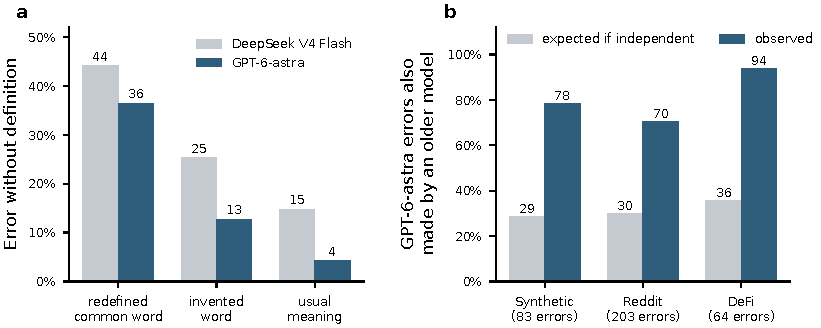
\includegraphics[width=.85\linewidth]{figs/phenomenon.pdf}
\caption{(a) Error without the definition on synthetic questions by designed term class. Familiar words given a new meaning are misread most often. (b) Share of GPT-6-astra's errors that another reader also makes on the same questions, against the share expected if errors were independent, which is the other readers' overall error rate on those questions (for DeFi, the rate at which DeepSeek V4.1 Flash or GPT-5.6-terra errs).}
\label{fig:phenomenon}
\end{figure}

The errors concentrate on familiar words given a new meaning. On synthetic terms whose local meaning conflicts with the usual one, DeepSeek V4 Flash errs on 44.2\% of questions, against 25.3\% on coined words and 14.8\% on words that keep their usual meaning. GPT-6-astra shows the same order, with 36.5\%, 12.7\%, and 4.2\% (Figure~\ref{fig:phenomenon}a). A familiar word misleads more than an unfamiliar one because the reader already has a confident reading of it. Table~\ref{tab:examples} shows three contract cases in which the usual meaning suggests a broader reading than the contract allows.

The errors are also stable. For 761 synthetic questions, DeepSeek V4 Flash gave a greedy answer and ten sampled answers at temperature 1.0. Of the 229 greedy errors, 93 (40.6\%) repeat the same wrong answer in all ten samples, and the majority answer is wrong for 142 (62\%). Majority voting would correct 38\% of greedy errors, but the errors that survive concentrate on redefined common words, where 65\% survive against 43\% on usual-meaning terms. A system that relies on agreement across samples \citep{self-consistency} removes the unstable errors and keeps the ones tied to local meaning.

Errors also overlap strongly across readers. On questions answered by every reader of a corpus, 78\% of GPT-6-astra's synthetic errors are also errors of DeepSeek V4 Flash, 70\% of its Reddit errors are also errors of DeepSeek V4.1 Flash, and 94\% of its DeFi errors are also made by DeepSeek V4.1 Flash or GPT-5.6-terra. If errors were independent, these shares would be 29\%, 30\%, and 36\% (Figure~\ref{fig:phenomenon}b). The readers differ in family and size, so this is not a controlled comparison of model generations, but it shows that the occurrences at risk depend on the text as much as on the model.
%
\section{The model's own confidence does not reveal the errors}
\label{sec:detect}
If misreadings came with uncertainty, the detectors already used to flag hallucinations would find them. We test three signals from the reader's own samples on the 456 synthetic questions shared with the proxy: disagreement among ten sampled answers, entropy of the sampled option distribution, and negative stated confidence \citep{selfcheckgpt,semantic-uncertainty,verbal-confidence}. None of them uses the answer key. For DeepSeek V4 Flash errors they reach AUROC 0.616 $[0.579, 0.656]$, 0.616 $[0.579, 0.656]$, and 0.617 $[0.558, 0.681]$ (Figure~\ref{fig:silent}a). On redefined common words they fall to 0.557, 0.557, and 0.463, against 0.60 to 0.72 on invented and usual-meaning terms (Appendix~\ref{app:signals-by-class}). The detectors fail precisely where local meaning is at stake. Our option-level entropy is narrower than semantic entropy over free-form answers \citep{semantic-entropy}, but the result agrees with the stability above. The small model's own uncertainty is no better. One minus its largest option probability reaches only 0.537 and 0.523 on redefined common words for the two readers.

Better calibration does not close the gap. Jev \citep{jev} is a decision model built to report calibrated confidence. Its confidence ranks its own errors without a definition with AUROC 0.643 on synthetic, 0.660 on Reddit, and 0.636 on CUAD questions, and with a model-drafted local gloss added, with 0.815, 0.790, and 0.868 (Figure~\ref{fig:silent}b). The same confidence channel works once the local meaning is present, an observation consistent with a limitation of information rather than calibration. A model cannot flag a meaning it does not know has changed, so confidence thresholds, abstention rules, and sample agreement tuned on ordinary errors pass these answers.

\begin{figure}[t]
\centering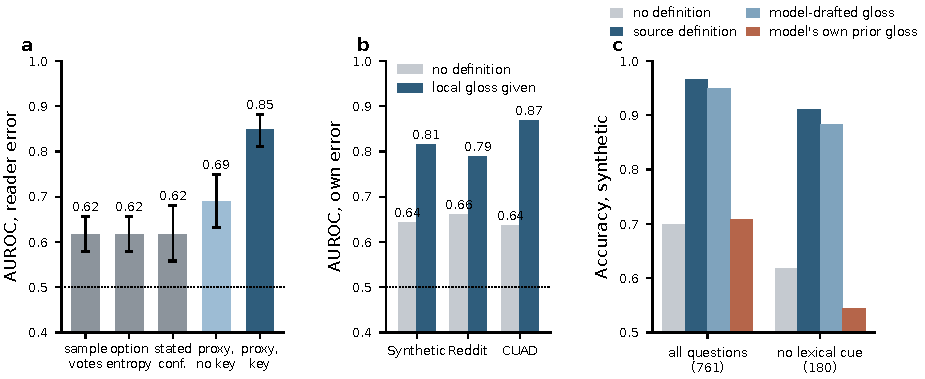
\includegraphics[width=\linewidth]{figs/silent_repair.pdf}
\caption{(a) AUROC for ranking DeepSeek V4 Flash errors on 456 synthetic questions, with 95\% intervals from resampling terms. Gray bars are key-free signals from the reader's ten samples and stated confidence. The light bar is the key-free uncertainty of the 7B proxy (one minus its largest option probability). The dark bar is the proxy score $R$, which checks the proxy against the source-implied answer. The dotted line marks chance. (b) Jev's native confidence as a detector of its own errors, without a definition and with a model-drafted local gloss. (c) DeepSeek V4 Flash accuracy on synthetic questions under four conditions: no definition, the source definition, a model-drafted gloss, and the model's own gloss of the term written under a domain prompt. The right group keeps only questions where no option is singled out by word overlap with any of the three texts.}
\label{fig:silent}
\end{figure}
%
\section{A small model predicts where frontier models fail}
\label{sec:predict}
\paragraph{Cross-reader prediction.}
The score $R$ uses a source-implied answer rather than asking whether the proxy feels uncertain. On the same 456 synthetic questions, Qwen2.5-7B $R$ ranks DeepSeek V4 Flash and GPT-6-astra errors with AUROC 0.848 and 0.809; on 1,500 stratified CUAD questions it ranks GPT-5.6-terra errors at 0.815 (Table~\ref{tab:prediction}). A different reader's observed answers are a reference for shared item difficulty, with AUROCs of 0.640--0.892 across settings (Appendix~\ref{app:reader-difficulty}). Thus the 7B proxy can give a useful review order without calling the target reader, but this comparison does not show that $R$ isolates local-meaning conflict. On synthetic questions discrimination rises from 0.699 at 0.5B to 0.848 at 7B and 0.867 at 14B. Reddit and DeFi provide five exploratory cross-reader settings (0.720--0.809), whose source and question-quality limits matter when interpreting the apparent portability.

\paragraph{Risk stratification across a contract library.}
We score 6,529 retained diagnostic questions from 303 CUAD contracts, then ask GPT-5.6-terra 300 questions from each of five risk bins. Observed error rises from 1.0\% in the lowest bin to 52.3\% in the highest (Figure~\ref{fig:strata}a). Reweighting to the scored frame gives a 13.2\% error rate and 0.846 AUROC. The top two bins contain 23\% of these questions and 66\% of their estimated errors. This is a concrete use for the index: a document owner can review high-risk source uses first, before a reader is deployed. The frame excludes occurrences without retained diagnostic questions, and cross-reader overlap is not a prospective test of the same index after an upgrade.

\begin{figure}[t]
\centering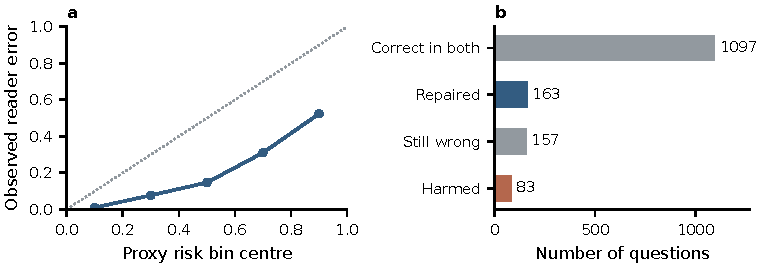
\includegraphics[width=.82\linewidth]{figs/stratification.pdf}
\caption{CUAD library validation with 300 questions per proxy risk bin and GPT-5.6-terra as reader. (a) Observed error rises with proxy risk. The dotted line marks equality, which the score does not attain because it ranks rather than estimates error. (b) Outcomes when the extracted contract definition is supplied. Repairs outnumber harms, and about half of the original errors remain.}
\label{fig:strata}
\end{figure}

\paragraph{What the score measures.}
$R$ also predicts errors that cannot be attributed to a conflicting local meaning. On synthetic terms retaining their usual meaning, its AUROC is 0.921 for DeepSeek V4 Flash and 0.846 for GPT-6-astra, based on 21 and 6 errors. On Reddit non-glossary controls it is 0.842 and 0.815 (Appendix~\ref{app:synthetic-control}). These controls make shared question difficulty a plausible component of the signal. The synthetic class comparison and definition interventions establish that local content matters in some questions, but $R$ alone cannot say \emph{why} a particular answer will be wrong. Its practical role is review triage, with the source definition and the question checked separately.

\paragraph{Question validity.}
Source-linked scores are only as credible as their keys. Two models screened 80 fixed-hash questions against available source material, after which an author reviewed 17 model-disagreement items and 10 stratified controls without seeing the keys. Subsequent source reconciliation classified 10 stored keys as supported, 14 questions as invalid or source-insufficient, and 3 as borderline. The selected 27 do not estimate a corpus-wide defect rate (Appendix~\ref{app:source-screen}, Table~\ref{tab:review}). Deleting the 14 clear problem items changes $R$ error AUROC by at most 0.00203 across the eight matched settings and leaves the synthetic 93/229 stable-error count unchanged. This local sensitivity says the \emph{found} problems do not drive those point estimates; it cannot validate unreviewed keys. We consequently treat synthetic and CUAD as the main controlled diagnostic evidence and Reddit and DeFi as exploratory transfers.

%
\section{Source-grounded definitions help, but text and scope matter}
\label{sec:repair}
\paragraph{Source content, not a prior-only gloss, drives the synthetic gain.}
On 761 synthetic questions whose drafter saw usage sentences but not a definition, DeepSeek V4 Flash accuracy is 0.699 without a note, 0.966 with the source definition, 0.949 with a model-drafted gloss \emph{based on that source}, and 0.708 with the reader's own domain-conditioned gloss (Figure~\ref{fig:silent}c). The source definition repairs 209 errors and harms 6 previously correct answers; the prior-only gloss repairs 86 and harms 79. A model can therefore write a useful paraphrase when it has the source, but asking it to supply a missing local rule from its own prior does not reproduce that benefit. In the 180 questions where a lexical-overlap screen singles out no option from any of the three notes, source-definition accuracy still rises from 0.617 to 0.911, versus 0.544 with the prior gloss. This check reduces one answer-cue concern without removing all construction effects (Appendix~\ref{app:lexical-cues}). For a semantic layer, the object to preserve is the source-bound rule and its scope, not merely a fluent gloss of the term.

The ability to use a supplied rule is separately testable. On 1,244 human-written Inverse Scaling redefinition items \citep{inverse-scaling}, GPT-5.6-terra and GPT-6-astra follow the stated meaning on 95.0\% and 99.8\%; without it both use the usual meaning on about 98\%. DeepSeek V4.1 Flash follows the stated meaning on 63.0\%. The contrast separates failure to \emph{receive} a local rule from failure to \emph{follow} one, and shows why the two should not be collapsed into a single intervention claim.

\paragraph{A definition's wording changes both repairs and harms.}
On Reddit glossary questions, a model-drafted source-based gloss repairs 171 errors but harms 58 correct answers; the community entry repairs 243 and harms 9. The corresponding DeFi counts are 42/20 and 70/3. In both corpora the question writer saw the source entry, so this is an informative text-version comparison, not an independent estimate of definition quality. It warns that supplying an inaccurate or poorly scoped note can make an answer worse. For the narrower target of \emph{which known bare errors the same note repairs}, $\Delta p$ ranks outcomes with AUROC 0.712--0.983 across eight heterogeneous settings (Appendix~\ref{app:statistics}). That diagnostic is tied to the exact text and the evaluated question. On 215 Reddit terms, a drafted-gloss score predicts sibling-question repairs at 0.811 AUROC, while a score computed with the community entry reaches 0.600 $[0.475,0.717]$; the latter entry already repairs 126 of 147 bare errors, leaving only 21 nonrepairs to rank (Appendix~\ref{app:new}). Neither result establishes that $\Delta p$ can choose definitions for unseen user requests.

\paragraph{A definition is not always sufficient.}
In CUAD, extracted contract definitions repair 163 errors but harm 83 correct answers, raising accuracy from 0.787 to 0.840 (Figure~\ref{fig:strata}b). Of 320 original errors, 157 remain. A definition may depend on schedules or other clauses, the question may be defective, or the reader may still apply it incorrectly. An operational system should therefore retrieve the linked evidence and allow an unresolved case to remain unresolved; simply attaching every matched term note is not a guarantee of correctness.

\paragraph{Which definitions to curate first.}
The cost of a definition library lies in writing, checking, and maintaining entries. In a 215-term Reddit development comparison at 25\% of total definition words, frequency-based selection has point estimates 3.5 and 4.5 accuracy points above frequency times mean $\Delta p$ for the two readers on policy-disagreement terms. Source-check uncertainty gives a difference interval of $[-9.21,+6.14]$ points, so neither policy is established as better. A small CUAD comparison also does not favour mean $\Delta p$ (Appendix~\ref{app:new}). The historical retrieval gains cannot establish advance selection because the evaluated question contributed to its own term score and the CUAD leave-one-question-out gain is only partially identified (Appendix~\ref{app:interventions}). For now, term frequency is a transparent default for deciding what to curate first; $R$ can separately order diagnostic questions for review. These are different decisions and should not be conflated.

%
\section{Implications of the Findings}
\label{sec:discussion}
\paragraph{A class of error that current evaluations do not measure.}
Error taxonomies for language models ask whether an answer contradicts the world or contradicts the input \citep{space}. Silent misreadings do neither. The input is consistent with the answer but incomplete relative to the document it came from, and the answer is wrong only with respect to that document. Such errors become visible only when an answer is compared with the full source rather than with the supplied input, and the small effect on public benchmarks indicates that this comparison is rarely made rather than that the errors are rare. Evaluations of systems that read local text, including retrieval-augmented generation, need questions that reach the boundaries of local definitions.

\paragraph{Knowing that a definition is needed is a distinct capability.}
Models largely know what they know \citep{know-what-know}, and calibration and selective prediction exploit this to abstain when uncertain \citep{calibration,selective}. A redefined common word defeats this mechanism, because the model is not uncertain about the word. It is confident in the wrong sense. The strongest readers follow a stated definition on nearly every item and misread largely the same occurrences as other readers, so the remaining failure is not a lack of capacity to use local meaning. It is the absence of any internal signal that local meaning is needed. Recognizing that a familiar word may carry a local meaning is thus a capability that neither scale nor calibration has produced, and a natural target for evaluation and training.

\paragraph{Designing systems that read local text.}
Three design consequences follow. Local definitions should be taken from the source rather than generated by the model. Safeguards based on confidence or sample agreement, and faithfulness-oriented decoding, should not be expected to catch these errors. In documents whose definitions refer to other material, retrieval must follow those references. The same considerations apply wherever text is written for a group whose vocabulary differs from general usage, as in software engineering terminology \citep{se-terminology}, community slang \citep{informal-language}, and organizational documents. Whether item-level difficulty rankings such as $R$ transfer to requests written by users is a direction for future work.
%
\section{Limitations and conclusion}
\label{sec:conclusion}
The questions are model-drafted, forced-choice diagnostics rather than independent user requests. The selected source review found invalid and insufficient items, especially in the reviewed CUAD and DeFi cases; its counts cannot estimate defect prevalence. Removing those found items barely changes the reported AUROCs, but unreviewed keys remain a threat. $R$ also predicts errors on usual-meaning and control terms, so it cannot identify an error's semantic cause by itself. The definition-allocation experiments are too limited to show an advantage over frequency, and the historical retrieval comparison is not a held-out request test.

The supported implication is a division of labour for systems that use local documents. At corpus preparation time, source-linked diagnostic questions can rank uses for human checking without asking every deployed reader to discover its own missing context. The checked definition should remain attached to its source and scope, because its wording changes both repairs and harms. At request time, retrieval still has to bring in the relevant definition and any linked clauses; the present score is not a substitute for that step. Evaluations should test missing local evidence as well as conflicts with evidence already shown. This is a useful offline diagnostic and a concrete design requirement for a semantic layer, while the benefit of an automatic definition-selection policy on new requests remains to be demonstrated.
\label{main:end}

%
\section*{Reproducibility statement}
We release a risk index over 6,529 retained CUAD diagnostic questions, 1,500 of them with frontier-reader outcomes, together with question sets, reader outcomes, proxy scores, and an experimental command-line pipeline for new corpora. The package includes model records, analysis scripts, and verification of the main numerical results. The appendix specifies each evaluation unit and the limits of the source review.
%
\subsubsection*{AI use statement}
We used generative AI tools to help develop theoretical models or conceptual frameworks, design or provide feedback on research methodology or experiments, implement code, assist with translation, clean and reformat datasets, interpret results, and support qualitative and thematic data analysis. We have not used generative AI tools to formulate mathematical claims, provide critical ingredients for proving mathematical claims, assist in the writing of proofs, propose or refine hypotheses. We have reviewed all AI-assisted work. We take responsibility for the final content of this work, including text, claims, or artifacts produced with the aid of generative AI.
%
\bibliography{references}
\bibliographystyle{iclr2027_conference}
\clearpage\appendix
\section{Data and question construction}
\label{app:sources}
Diagnostic questions are generated from source passages and local definitions. A question specifies an option set and a source-grounded answer key. These keys support behavioural measurement but do not constitute expert adjudication of every application scenario. The supplementary inventory distinguishes question-level results from term-level means and keeps separate task versions separate.

\paragraph{Synthetic vocabulary.}
The source design uses invented trading-desk and restaurant-group vocabulary. Categories and local definitions are specified before text generation, and the diagnostic intervention uses a model-drafted gloss derived from the source. The archived uncertainty experiment contains 763 questions from 197 nonempty term records. Excluding two questions affected by a source-definition conflict leaves 761 for analysis. The archived 7B proxy overlap has 457 questions from 119 records. Excluding its one affected question leaves 456. The usage-based inline experiment contains 965 questions. Frequency is deliberately varied in the synthetic design, so rarity comparisons concern that design rather than a natural corpus distribution.

\paragraph{CUAD.}
The source corpus contains 510 contracts. Extraction retains 2,174 term records in 303 contracts and identifies 24,880 candidate occurrences. Question drafting and per-term caps yield a 6,529-question scored frame. The stratified validation sample contains 1,500 questions in 1,012 term records and 215 contracts. A separate definition-anchored task contains 671 questions in 187 terms. These task sets have different construction rules and are analysed separately.

The introductory example is record \texttt{cuadfull:379:Trademarks}, question at context index 2. Its definition restricts Trademarks to the trademarks and trade names identified in Exhibit~A. The usage requires the distributor to notify the manufacturer of unauthorized use of the Trademarks, so the notification duty covers only the listed names.

\paragraph{Reddit.}
The data contain 393 term records, of which 352 have questions. The 1,391 retained questions span 35 communities. The RAG workload contains 851 glossary-word questions and 540 control-word questions. All 393 stored diagnostic \texttt{gloss\_used} fields are marked as model drafted. Among the 218 glossary terms with a source entry, none of these drafted texts equals \texttt{gloss\_gold}. Controls need not have a source entry. A comparison involving \texttt{gloss\_used} therefore measures that rewrite, not the community source entry alone.

\paragraph{DeFi.}
The set contains 379 questions from 97 nonempty term records. It tests technical vocabulary in DeFi documentation. All 98 stored candidate glosses are model drafted and differ from the recorded source glosses. Official model cards give knowledge cutoffs of February 16, 2026 for \texttt{gpt-5.6-terra} and April 30, 2026 for \texttt{gpt-6-astra} \citep{openai-gpt56-terra-model,openai-gpt6-astra-model}. The collected documentation snapshot contains later file dates, but each term links a median of 18 documents and questions have no verified first-publication date for their answer-bearing rule. Uniswap v4 and Unichain were public in 2025 \citep{uniswap-v4-launch,unichain-launch}. Thus the GPT readers' $R$ AUROCs of 0.792 and 0.764 measure cross-reader error ranking on these questions. They do not rule out knowledge of earlier documentation or prove that answers were not memorized. The analysis does not depend on an assumption that this material was absent from model training.

\paragraph{Question and answer-key validity.}\label{app:source-screen}
A fixed SHA-256 rule selected 20 historical questions from each corpus before comparing any new answers with the stored keys. Reddit was split evenly between its ordinary question frame and a frozen strategy-disagreement frame. This 10/10 split is not a natural prevalence estimate. DeepSeek V4.1 Flash and Claude Sonnet 5 independently read the same source cards and question-only excerpts from linked documents. Both were run without explicit reasoning. DeepSeek used temperature zero and a 550-token output cap. Sonnet 5 rejected temperature zero, so its host used the provider default and a 1,000-token cap. All 80 Sonnet responses ended normally, but its host did not expose provider response IDs. The models saw neither the stored key nor reader outcomes. Long contracts and DeFi documents were excerpted, and the Reddit archive preserves glossary entries and selected comments rather than every complete original post.

\begin{table}[h]\centering\small
\caption{Model source screening on 20 questions per corpus. ``Both key'' means both models gave a unique source-supported answer matching the stored key. ``Both other'' means they agreed on another answer. ``Split answer'' means two supported but different answers. ``One supported'' means one model judged the source sufficient and the other did not. ``Neither supported'' includes insufficient or ambiguous evidence. These are screening categories, not expert answer-key error rates.}
\label{tab:source-screen}
\begin{tabular}{@{}lrrrrr@{}}\toprule
Corpus & Both key & Both other & Split answer & One supported & Neither supported\\\midrule
Synthetic & 18 & 0 & 0 & 1 & 1\\
CUAD & 13 & 1 & 1 & 4 & 1\\
Reddit & 3 & 0 & 0 & 3 & 14\\
DeFi & 5 & 0 & 0 & 7 & 8\\\bottomrule
\end{tabular}
\end{table}

\paragraph{Human source review.}
From the 80 fixed-hash questions, an author answered 27 from the available source before seeing the stored key. Seventeen were model-screen disagreement cases; ten were sampled within corpus and screen categories. The author selected an option on 11 and marked 16 undetermined. A different letter was not automatically counted as a key error: the local definition supports the stored key in some such cases. Subsequent source reconciliation, conducted after viewing the key, produced Table~\ref{tab:review}; it is not an independent blinded second annotation and yields no agreement coefficient.
\begin{table}[h]\centering\footnotesize
\caption{Source review of 27 selected diagnostic questions: 17 model-screen disagreements and ten stratified controls. Counts describe this enriched sample, not corpus-wide defect rates.}
\label{tab:review}
\begin{tabular}{@{}lcccc@{}}\toprule
Corpus & Key supported & Invalid or source-insufficient & Borderline & Reviewed\\\midrule
Synthetic & 3 & 1 & 0 & 4\\
CUAD & 2 & 6 & 1 & 9\\
Reddit & 3 & 1 & 1 & 5\\
DeFi & 2 & 6 & 1 & 9\\\midrule
Total & 10 & 14 & 3 & 27\\\bottomrule
\end{tabular}\end{table}

The reviewed defects include a redacted exhibit needed to determine a manufacturer's duty, an item with literal A/B/C/D placeholders as its options, a mandatory-removal question where the contract permits removal, and a blocked-swap status with two possible causes. In one CUAD item the stored option names user guides and technical manuals as rights not granted, although the contract explicitly grants rights to Documentation; the item was removed rather than rekeyed using probabilities computed for the old answer. Conversely, the community entries for \emph{Fill}, \emph{Burst}, and \emph{Standard} can resolve constructed Reddit scenarios without an archived post describing that exact scenario. These distinctions require source reading rather than equating an author-model disagreement with a wrong key.
\begin{table}[h]\centering\footnotesize
\caption{Deletion sensitivity after removing the 14 reviewed questions classified as clearly invalid or source-insufficient. Other questions retain their historical keys. This is a local sensitivity analysis, not a validated-only re-estimate. $\Delta p$ AUROC targets repair among observed bare errors on the same question.}
\label{tab:validity-sensitivity}
\begin{tabular}{@{}p{4.0cm}rcc@{}}\toprule
Setting & Items retained & $R$ error AUROC & Conditional repair $\Delta p$ AUROC\\\midrule
Synthetic / DeepSeek V4 Flash & 455/456 & .848 $\to$ .847 & .983 $\to$ .983\\
Synthetic / GPT-6-astra & 455/456 & .809 $\to$ .809 & .962 $\to$ .962\\
Reddit / DeepSeek V4.1 Flash & 1,390/1,391 & .808 $\to$ .808 & .858 $\to$ .860\\
Reddit / GPT-6-astra & 1,390/1,391 & .720 $\to$ .720 & .812 $\to$ .812\\
DeFi / DeepSeek V4.1 Flash & 373/379 & .809 $\to$ .808 & .863 $\to$ .863\\
DeFi / GPT-5.6-terra & 373/379 & .792 $\to$ .791 & .794 $\to$ .794\\
DeFi / GPT-6-astra & 373/379 & .764 $\to$ .764 & .846 $\to$ .852\\
CUAD / GPT-5.6-terra & 1,494/1,500 & .815 $\to$ .817 & .712 $\to$ .714\\\bottomrule
\end{tabular}
\end{table}

Removing the 14 clearly invalid or source-insufficient reviewed items changes $R$ error-ranking AUROC by at most 0.00203 and same-question repair $\Delta p$ AUROC by at most 0.00601 across the eight matched settings. CUAD design-weighted $R$ AUROC changes from 0.8456 to 0.8467, and the corrected synthetic repeated-sampling count remains 93 identical wrong answers among 229 greedy errors. Removing the three borderline items as well has little effect on these point estimates. The 17 targeted items and ten stratified controls are not a random draw from all historical questions; their category counts are not defect rates. Most historical questions remain unreviewed, and this local deletion check cannot validate them. The 24 items in the original 80 for which neither screening model found a source-supported unique answer remain unresolved rather than being treated as wrong keys.

\paragraph{Definition version by CUAD task.}
The 1,500-question CUAD library builds its proxy and reader definition arm from \texttt{def\_raw}, the extracted contract wording. The distinct 671-question definition-anchored CUAD package instead has an automatically drafted \texttt{glossC} arm and a separate original-contract \texttt{glossG} arm. All 204 small-package term records mark \texttt{gloss\_used} as drafted and different from the source entry. Archived per-question prompts confirm that all 671 \texttt{glossC} notes match the drafted text and all 671 \texttt{glossG} notes match the original-contract text. These CUAD tasks must not be described as one common definition intervention.

\paragraph{Eight nonexchangeable reader settings.}\label{app:setting-design}
Table~\ref{tab:setting-design} records the reader alias, intervention text, and information visible to the question drafter. The synthetic questions were drafted from usage contexts without the source definition in the drafting prompt. Reddit and DeFi questions were drafted with their source entries, which also informed answer keys. The later reader intervention supplied a different model-drafted gloss. CUAD questions were drafted from an extracted contract definition and one usage occurrence. Within a corpus, additional readers answered the same diagnostic questions. Across corpora, the question construction and definition versions differ. The rows cannot be pooled as replications of one fixed data-generating process.

\begin{table}[h]\centering\footnotesize
\caption{Reader settings in Table~\ref{tab:prediction}. Synthetic DeepSeek calls used V4 Flash. Later calls used V4.1 Flash. DeepSeek documents the API IDs \texttt{deepseek-v4-flash} and \texttt{deepseek-flash}, respectively. ``Source entry'' describes drafting input and does not imply that the reader's \texttt{glossC} arm used that entry.}
\label{tab:setting-design}
\begin{tabular}{@{}>{\raggedright\arraybackslash}p{1.5cm}>{\raggedright\arraybackslash}p{3.0cm}>{\raggedright\arraybackslash}p{3.4cm}>{\raggedright\arraybackslash}p{4.7cm}@{}}\toprule
Corpus & Reader API alias & Definition given to reader & Question drafting input\\\midrule
Synthetic & DeepSeek V4 Flash & Model-drafted \texttt{glossC} & Invented-term usage contexts. No source definition in drafting prompt\\
Synthetic & \texttt{gpt-6-astra} & Model-drafted \texttt{glossC} & Same synthetic questions\\
Reddit & DeepSeek V4.1 Flash & Model-drafted \texttt{glossC} & Community glossary entry and comment contexts\\
Reddit & \texttt{gpt-6-astra} & Model-drafted \texttt{glossC} & Same Reddit questions\\
DeFi & DeepSeek V4.1 Flash & Model-drafted \texttt{glossC} & Source glossary entry and documentation contexts\\
DeFi & \texttt{gpt-5.6-terra} & Model-drafted \texttt{glossC} & Same DeFi questions\\
DeFi & \texttt{gpt-6-astra} & Model-drafted \texttt{glossC} & Same DeFi questions\\
CUAD & \texttt{gpt-5.6-terra} & Extracted contract \texttt{def\_raw} & One definition and one contract usage per question\\\bottomrule
\end{tabular}
\end{table}

\paragraph{Designed-class control for mechanism specificity.}\label{app:synthetic-control}
The synthetic vocabulary assigns terms to prior-conflict, prior-consistent, and no-ordinary-prior classes before generating diagnostic questions. Table~\ref{tab:synthetic-control} evaluates $R$ against reader bare errors separately in each class, with term-record bootstrap intervals. The score ranks errors in the prior-consistent class, where a conflicting usual meaning was not designed into the term. It also ranks errors for terms with no ordinary prior. These findings show that the observed error-ranking performance is not specific to meaning conflict. The classes are synthetic design labels, not independent diagnoses of each error, and the GPT-6-astra prior-consistent row has only six errors.

\begin{table}[h]\centering\small
\caption{Error-ranking $R$ by designed synthetic term class. Reader cells give errors, AUROC [95\% CI]. Both readers answer the same 456 questions. Intervals resample term records.}
\label{tab:synthetic-control}
\begin{tabular}{@{}lrrr@{}}\toprule
Class & Questions & DeepSeek V4 Flash & GPT-6-astra\\\midrule
Prior conflict & 156 & 69, 0.803 [0.739, 0.864] & 57, 0.777 [0.697, 0.854]\\
Prior consistent & 142 & 21, 0.921 [0.870, 0.966] & 6, 0.846 [0.710, 0.993]\\
No ordinary prior & 158 & 40, 0.779 [0.704, 0.849] & 20, 0.720 [0.629, 0.819]\\\bottomrule
\end{tabular}
\end{table}

\paragraph{Reddit non-glossary controls.}
The Reddit workload also contains 540 questions attached to terms outside the community glossary. DeepSeek V4.1 Flash has 0.235 bare-error rate and $R$ AUROC 0.842 on these controls, versus 0.343 and 0.781 on 851 glossary-term questions. GPT-6-astra has corresponding control values 0.143 and 0.815, versus 0.148 and 0.659 on glossary terms. The non-glossary terms are a useful difficulty reference, but absence from the collected glossary does not prove absence of every local sense. The separate source audit also finds substantial Reddit question-answerability uncertainty.

\paragraph{Other readers as a difficulty reference.}\label{app:reader-difficulty}
On identical questions, another reader's observed bare correctness can serve as a coarse indication of shared item difficulty. Table~\ref{tab:reader-difficulty} compares that binary or two-reader error-count score with the continuous proxy $R$. The comparator uses another frontier model's answers and is therefore not a low-cost deployment baseline or a statistical upper bound. Its resolution differs from $R$, and both may respond to the same local-meaning failure. The proxy was not rescored with the source usage or target term removed. These measurements cannot isolate a semantic component of $R$.

\begin{table}[h]\centering\footnotesize
\caption{AUROC for predicting a target reader's bare errors on the same questions. ``Other readers'' is one observed reader error or the mean of two other reader errors. All models share the historical question and answer key.}
\label{tab:reader-difficulty}
\begin{tabular}{@{}llrcc@{}}\toprule
Corpus & Target reader & $n$ & Proxy $R$ & Other readers\\\midrule
Synthetic & DeepSeek V4 Flash & 456 & .848 & .722\\
Synthetic & GPT-6-astra & 456 & .809 & .804\\
Reddit & DeepSeek V4.1 Flash & 1,391 & .808 & .640\\
Reddit & GPT-6-astra & 1,391 & .720 & .736\\
DeFi & DeepSeek V4.1 Flash & 379 & .809 & .750\\
DeFi & GPT-5.6-terra & 379 & .792 & .867\\
DeFi & GPT-6-astra & 379 & .764 & .892\\\bottomrule
\end{tabular}
\end{table}

\paragraph{Stability and key-free signals by term class.}\label{app:signals-by-class}
Table~\ref{tab:signals-by-class} splits the synthetic stability and detection results by the designed term class. Stability columns use the 761-question sampling frame for DeepSeek V4 Flash. Detection columns use the 456 questions shared with the proxy, where error counts are smaller. Sample disagreement and option entropy give identical rankings on these ten-sample votes, so only disagreement is shown. The key-free proxy score is one minus the proxy's largest option probability, recomputed with the released scoring prompt. The rerun reproduces the stored keyed probabilities to within 0.005. Intervals resample term records.

\begin{table}[h]\centering\scriptsize\setlength{\tabcolsep}{3pt}
\caption{Synthetic stability and error-detection AUROC by term class for DeepSeek V4 Flash. ``Same wrong'' counts greedy errors repeated identically in all ten samples. ``Majority wrong'' counts errors that survive majority voting.}
\label{tab:signals-by-class}
\resizebox{\linewidth}{!}{\begin{tabular}{@{}lrrrrcccc@{}}\toprule
 & \multicolumn{3}{c}{Stability (761 questions)} & \multicolumn{5}{c}{Detection AUROC (456 questions)}\\\cmidrule(lr){2-4}\cmidrule(lr){5-9}
Class & Errors & Same wrong & Majority wrong & Errors & Disagreement & Stated conf. & Proxy, no key & Proxy $R$\\\midrule
Redefined common word & 168/461 & 74 (44\%) & 110 (65\%) & 69 & 0.557 [0.492, 0.622] & 0.463 [0.376, 0.554] & 0.537 [0.439, 0.636] & 0.803 [0.738, 0.864]\\
Coinage & 40/158 & 12 (30\%) & 23 (58\%) & 40 & 0.641 [0.570, 0.720] & 0.715 [0.637, 0.785] & 0.718 [0.615, 0.816] & 0.779 [0.704, 0.848]\\
Usual meaning & 21/142 & 7 (33\%) & 9 (43\%) & 21 & 0.603 [0.517, 0.692] & 0.644 [0.552, 0.730] & 0.810 [0.710, 0.897] & 0.921 [0.871, 0.965]\\
All & 229/761 & 93 (41\%) & 142 (62\%) & 130 & 0.616 [0.579, 0.656] & 0.617 [0.558, 0.681] & 0.689 [0.632, 0.750] & 0.848 [0.812, 0.881]\\
\bottomrule\end{tabular}}\end{table}

\begin{table}[h]\centering\footnotesize
\caption{Bare error and proxy $R$ AUROC by term class. Synthetic classes are fixed by the corpus design. Reddit glossary terms have a community entry, and control words are ordinary words from the same communities without one.}
\label{tab:classes}
\begin{tabular}{@{}llrcccc@{}}\toprule
 & & & \multicolumn{2}{c}{DeepSeek Flash} & \multicolumn{2}{c}{GPT-6-astra}\\\cmidrule(lr){4-5}\cmidrule(lr){6-7}
Corpus & Term class & $n$ & Error & $R$ AUROC & Error & $R$ AUROC\\\midrule
Synthetic & Redefined common word & 156 & 0.442 & 0.803 & 0.365 & 0.777\\
Synthetic & Coinage & 158 & 0.253 & 0.779 & 0.127 & 0.720\\
Synthetic & Usual meaning & 142 & 0.148 & 0.921 & 0.042 & 0.846\\
Reddit & Glossary term & 851 & 0.343 & 0.781 & 0.148 & 0.659\\
Reddit & Control word & 540 & 0.235 & 0.842 & 0.143 & 0.815\\\bottomrule
\end{tabular}\end{table}


%
\section{Scoring and statistical methods}
\label{app:statistics}
\paragraph{Answer-label scores.}
The diagnostic proxy normalises scores across answer letters. The seven proxy tokenizers represent both the plain and space-prefixed A/B/C/D labels with one token per spelling, without cross-letter token collisions. The historical estimator takes the higher score over these two spellings for each letter. This convention defines the proxy score and is not a claim of calibrated reader confidence. Model and tokenizer revisions appear in Appendix~\ref{app:models}.

The signed probability change $\Delta p$ is defined in Equation~\ref{eq:gain}. It is indexed by the exact definition text, its scope and its version. A mean log-score contrast, stored as \texttt{delta\_mc} in the supplementary data, is a separate statistic and is not substituted for $\Delta p$.

\paragraph{Pairing and evaluation units.}
Prediction comparisons match record IDs and question stems, with context indices for the CUAD library. Reader records specify answer keys and option order. The main table reports question-level outcomes. Term-level Sonnet summaries have a different unit and remain in the supplementary inventory.

\paragraph{Definition-anchored CUAD task.}
On 671 matched questions, bare accuracy is 0.772 and accuracy with the \emph{drafted} \texttt{glossC} is 0.903. The separate original-contract \texttt{glossG} arm reaches 0.982, and its correctness differs from \texttt{glossC} on 57 items. Error-ranking AUROC is 0.858 for $R$ and 0.666 for $\Delta p$ computed with the drafted gloss. These proxy probabilities do not measure the response to the contract text. This task is distinct from the 1,500-question usage validation.

\paragraph{Stratified validation.}
The five CUAD risk strata contain 2,529, 1,430, 1,085, 980, and 505 scored questions. A seeded shuffle with seed 42 selects 300 questions per stratum. The inverse inclusion weight is the stratum population divided by 300. Weighted error AUROC uses weighted positive-negative pairs. Within the 6,529-question frame, the weighted failure rate is 13.2\%, $R$ AUROC is 0.846, and $\Delta p$ AUROC is 0.500. These weights do not cover occurrences excluded during question construction.

\paragraph{Uncertainty intervals.}
Primary intervals use 2,000 cluster-bootstrap replicates. Paired arms share each resample. CUAD clusters are contracts, Reddit clusters are communities, and synthetic and DeFi comparisons use term records. The intervals quantify variation across the observed clusters, not across arbitrary organisations, question generators, or repeated model calls. Exploratory subgroup and threshold results are interpreted separately from primary comparisons.

The Synthetic / GPT-6-astra and DeFi / DeepSeek V4.1 Flash rows in Table~\ref{tab:prediction} round to the same $R$ point estimate and interval at three decimal places. Their unrounded values differ: 0.8094577 with interval $[0.7627638,0.8560215]$ and 0.8093046 with $[0.7625671,0.8555733]$, respectively. The duplicate printed values result from rounding under the manuscript's original bootstrap procedure, rather than copying one row into the other. A separate bootstrap seed changes finite-replicate endpoints slightly and is not substituted into only one row.

\paragraph{Repair prediction.}
Table~\ref{tab:repair} evaluates prediction of a wrong-to-correct transition after a definition. Its final column reports a paired interval for the difference between the two scores on the separate bare-error target.
\begin{table}[t]\centering\footnotesize
\caption{Prediction of observed repair. The last column concerns the separate bare-error target and gives a paired ranking difference. $R$ and $\Delta p$ are algebraically coupled (Appendix~\ref{app:coupling}).}
\label{tab:repair}
\begin{tabular}{@{}p{4.5cm}rccc@{}}\toprule
Setting & $n$ & $R$, repair AUC & $\Delta p$, repair AUC & Error AUC difference CI\\\midrule
Synthetic / DeepSeek V4 Flash & 456 & 0.833 & 0.810 & [-0.168, -0.046]\\
Synthetic / GPT-6-astra & 456 & 0.797 & 0.716 & [-0.259, -0.066]\\
Reddit / DeepSeek V4.1 Flash & 1391 & 0.744 & 0.709 & [-0.323, -0.244]\\
Reddit / GPT-6-astra & 1391 & 0.725 & 0.621 & [-0.364, -0.213]\\
DeFi / DeepSeek V4.1 Flash & 379 & 0.769 & 0.686 & [-0.445, -0.251]\\
DeFi / GPT-5.6-terra & 379 & 0.792 & 0.556 & [-0.502, -0.327]\\
DeFi / GPT-6-astra & 379 & 0.754 & 0.590 & [-0.510, -0.324]\\
CUAD library / GPT-5.6-terra & 1500 & 0.760 & 0.595 & [-0.395, -0.302]\\
\bottomrule\end{tabular}\end{table}
\paragraph{Algebraic coupling of error risk and definition response.}\label{app:coupling}
Let $p_0$ and $p_d$ be the proxy probabilities assigned to the keyed option without and with the supplied definition. By construction, $R=1-p_0$ and $\Delta p=p_d-p_0=R+p_d-1$. Because $0\leq p_d\leq1$, the two scores satisfy $R-1\leq\Delta p\leq R$. They are therefore neither algebraically nor statistically independent. The paired bootstrap interval in Table~\ref{tab:repair} compares their rankings on the same bare-error target. Pairing handles shared sampling variation but does not remove this structural dependence. It is not evidence that $\Delta p$ isolates a distinct cause of error.

\begin{table}[h]\centering\footnotesize
\caption{Why $\Delta p$ can rank bare-reader errors below chance. Means are listed as bare-error / bare-correct items. The final column compares only error--correct pairs inside the same proxy-$R$ decile, a descriptive approximate control for the common $p_0$ term. It is not a causal decomposition.}
\label{tab:dp-coupling}
\begin{tabular}{@{}lcccc@{}}\toprule
Setting & $\Delta p$ error AUC & Mean $p_d$ & Mean $\Delta p$ & Within-$R$-decile AUC\\\midrule
Synthetic / DeepSeek V4 Flash & 0.745 & .804 / .924 & .496 / .246 & .485\\
Synthetic / GPT-6-astra & 0.656 & .751 / .920 & .450 / .287 & .431\\
Reddit / DeepSeek V4.1 Flash & 0.520 & .440 / .675 & .163 / .131 & .409\\
Reddit / GPT-6-astra & 0.429 & .405 / .639 & .105 / .147 & .359\\
DeFi / DeepSeek V4.1 Flash & 0.458 & .410 / .670 & .116 / .130 & .411\\
DeFi / GPT-5.6-terra & 0.380 & .356 / .668 & .064 / .144 & .307\\
DeFi / GPT-6-astra & 0.342 & .330 / .651 & .034 / .144 & .273\\
CUAD / GPT-5.6-terra & 0.464 & .407 / .714 & .139 / .141 & .398\\\bottomrule
\end{tabular}
\end{table}

For the bare-error target, a $\Delta p$ AUROC below 0.5 means that low definition response tends to accompany observed errors. In DeFi / GPT-6-astra, for example, mean $R$ is 0.704 for bare errors and 0.494 for bare-correct items, but mean post-definition support $p_d$ is 0.330 versus 0.651. The post-definition difference more than offsets the risk difference, leaving mean $\Delta p$ at 0.034 versus 0.144. The CUAD means nearly cancel, while pairwise ranks still give AUROC 0.464. A weak or negative association with \emph{bare error} does not contradict a positive association with \emph{repair conditional on bare error}, because those are different prediction targets. The within-decile values remain descriptive: they do not control item difficulty beyond $R$, question construction, or source-key quality.

The more specific target restricts evaluation to a reader's bare failures and asks which of those errors the same definition fixes. Table~\ref{tab:conditional-repair} gives direct and within-term sibling estimates for the recorded intervention text. Conditional results cannot by themselves guide pre-answer selection, because bare failure is then unknown.
\begin{table}[t]\centering\footnotesize
\caption{Predicting repair among the reader's bare failures. $R$ and $\Delta p$ use the same diagnostic item in the middle columns. The last column uses other scored questions of the same term record, with the available failed-question count in parentheses. CUAD uses the full proxy-scored frame for sibling estimates. Other rows use their available scored siblings. The CUAD 95\% interval is $[0.494,0.661]$.}
\label{tab:conditional-repair}
\begin{tabular}{@{}p{4.4cm}rccc@{}}\toprule
Setting & Bare failures & $R$ & $\Delta p$ & Other-item $\Delta p$ ($n$)\\\midrule
Synthetic / DeepSeek V4 Flash & 130 & 0.445 & 0.983 & 0.914 (130)\\
Synthetic / GPT-6-astra & 83 & 0.421 & 0.962 & 0.976 (83)\\
Reddit / DeepSeek V4.1 Flash & 419 & 0.453 & 0.858 & 0.824 (418)\\
Reddit / GPT-6-astra & 203 & 0.554 & 0.812 & 0.864 (203)\\
DeFi / DeepSeek V4.1 Flash & 107 & 0.501 & 0.863 & 0.850 (107)\\
DeFi / GPT-5.6-terra & 87 & 0.568 & 0.794 & 0.799 (87)\\
DeFi / GPT-6-astra & 64 & 0.476 & 0.846 & 0.874 (64)\\
CUAD / GPT-5.6-terra & 320 & 0.462 & 0.712 & 0.581 (190)\\
\bottomrule\end{tabular}\end{table}


\paragraph{Question-independent meaning difference.}\label{app:meaning-difference}
We separately measure how unlike a local definition is from a model's prior gloss of the term. The uncontextualized distance is $1-\cos(e(d_{\mathrm{source}}),e(g_{\mathrm{prior}}))$, where $e$ is the reported BAAI/bge-base-en-v1.5 sentence encoder \citep{bge}. A second distance uses the model's domain-conditioned prior gloss. Model self-report scores ask whether the term has a special use in the corpus, and model-assigned relation labels include \emph{none}, \emph{narrower}, and \emph{shifted}. These measurements do not use a diagnostic question. For contrast, we also show a term-mean comparison of an automatically drafted local gloss against an elicited prior gloss, together with term-mean $\Delta p$ and $R$. Those three scores do use diagnostic questions. Distances are unavailable when the model returned an unknown prior gloss.

\begin{table}[h]\centering\small
\caption{Distinguishing designed redefinitions from usual-meaning terms in the synthetic vocabulary, after excluding one source-definition-conflicted term. Each score uses all available terms for that score. Coverage differs and point estimates should not be ranked as if measured on one common sample. The class label was fixed by construction.}
\label{tab:term-difference-synthetic}
\begin{tabular}{@{}lccc@{}}\toprule
Term score & Uses questions? & Terms (shifted / consistent) & Class AUROC\\\midrule
No-context definition distance & No & 66 (38 / 28) & 0.946\\
Domain-prior definition distance & No & 157 (118 / 39) & 0.977\\
Model self-report & No & 79 (40 / 39) & 0.984\\
Drafted-local/prior answer contrast & Yes & 78 (40 / 38) & 0.917\\
Mean $\Delta p$ & Yes & 78 (40 / 38) & 0.783\\
Mean $R$ & Yes & 78 (40 / 38) & 0.817\\\bottomrule
\end{tabular}
\end{table}

The strong synthetic separation is a positive control for a deliberately designed semantic contrast, not an estimate of real-corpus misreading. To compare a source-definition distance with reader behaviour, we use only the archived reader arm that supplied that same source definition, \texttt{glossG}. A term's repair rate is the fraction of its historical questions answered wrongly without a definition and correctly with \texttt{glossG}. This term-level outcome uses a median of four questions per term. The automatically drafted \texttt{glossC} arm would compare a different intervention text and is excluded from this alignment.

\begin{table}[h]\centering\small
\caption{Spearman association of question-independent term scores with source-definition repair rate. Parentheses give available terms. Distance confidence intervals resample term records. There is no aligned \texttt{glossG} reader arm for this 204-term CUAD package. Only 54 terms have an uncontextualized prior gloss.}
\label{tab:term-difference-repair}
\begin{tabular}{@{}lccc@{}}\toprule
Corpus & No-context distance [95\% interval] & Domain-prior distance & Self-report\\\midrule
Synthetic & $0.452$ $[0.260,0.602]$ (65) & $0.300$ (186) & $0.465$ (118)\\
Reddit & $0.181$ $[0.046,0.303]$ (211) & $0.095$ (217) & $0.166$ (217)\\
DeFi & $-0.087$ $[-0.361,0.186]$ (57) & $0.101$ (64) & $-0.237$ (64)\\\bottomrule
\end{tabular}
\end{table}

The direct version-aligned test of the proposed term-level link uses the Reddit proxy's archived scores with the exact community entry. On 209 terms with 418 A questions, no-context distance has Spearman correlation $0.188$ with the term's mean source-definition $\Delta p$, with a term-bootstrap interval $[0.047,0.323]$. This is a weak positive association, not evidence that meaning difference is absent. It cannot identify which future question falls on a decision boundary. Both this proxy test and the repair test still use historical model-drafted questions, and the separate source audit finds substantial answerability uncertainty for Reddit and DeFi.

Model-assigned relation labels also give weak and inconsistent repair separation on the source-definition arm. Among Reddit glossary terms, 186 labelled \emph{narrower} or \emph{shifted} have mean repair rate 0.292, versus 0.266 for 31 labelled \emph{none}. The term-level repair AUROC is 0.531. In DeFi, the corresponding rates are 0.227 versus 0.333 over 32 terms per group, with AUROC 0.411. These are model-assigned lexical relations, not independent annotations of the three situations in Table~\ref{tab:cases}. A single text distance cannot by itself tell whether a use involves meaning conflict, an unspecified local scope, or missing information elsewhere. The synthetic reader-aligned text pairs and embedding script are retained, and the other source/prior texts remain in the archived weights. The exact BGE revision and embedding vectors are not, so exact bitwise reproduction of the cosine values is not guaranteed. The reported associations and source-aligned reader outcomes are reproducible from the archived scores.


\paragraph{Sampling consistency.}
The archived synthetic uncertainty experiment contains ten sampled responses per question, for 7,630 answer letters, and a separate greedy response. After removing the two source-conflicted questions, the analysis uses 761 questions and 7,610 of the archived letters. Among 229 greedy errors, 154 have ten identical sampled answers. Of these, 93 are identical and wrong, while 61 are identical and correct. The majority sampled answer is wrong on 142 of the 229 items. The corrected common proxy comparison uses 456 questions. Entropy is computed over option votes, and elicited confidence is treated as a response measurement rather than a calibrated probability.

%
\section{Definition interventions}
\label{app:interventions}
\begin{table}[h]\centering\footnotesize
\caption{DeepSeek Flash readers on matched historical four-arm questions: V4 for synthetic and V4.1 for Reddit and DeFi. Cell values are accuracy, followed by repairs/harms relative to bare. \texttt{glossG} is the source definition, \texttt{glossC} the model-drafted local gloss, and \texttt{glossM} a domain-conditioned prior gloss elicited without the source examples. The synthetic row excludes two source-conflicted questions. Reddit and DeFi drafters saw the source definition, so these are constructed-task interventions rather than independent downstream uses.}
\label{tab:definition-arms}
\begin{tabular}{@{}lrrrrr@{}}\toprule
Corpus & $n$ & Bare & Source \texttt{glossG} & Drafted \texttt{glossC} & Domain-prior \texttt{glossM}\\\midrule
Synthetic & 761 & .699 & .966 (209/6) & .949 (196/6) & .708 (86/79)\\
Reddit glossary & 851 & .657 & .932 (243/9) & .790 (171/58) & .616 (82/117)\\
DeFi source-entry & 250 & .672 & .940 (70/3) & .760 (42/20) & .740 (40/23)\\\bottomrule
\end{tabular}
\end{table}

\paragraph{Lexical shortcuts in generated questions.}\label{app:lexical-cues}
The diagnostic questions and local glosses can share words even when the question does not quote the gloss verbatim. A simple warning rule removes the target term and common English words, then chooses the option with the unique largest fraction of content words overlapping the exact drafted \texttt{glossC}. The synthetic \texttt{raw\_outputs} glosses match all 197 recovered reader term prompts. A different same-named input file does not. Table~\ref{tab:lexical-cues} reports how often this rule selects the stored key. A shuffled-gloss baseline permutes glosses among terms within the corpus. The reader's own question is retained in the no-cue subset, but a missing lexical flag is not a semantic proof that no answer leakage remains.

\begin{table}[h]\centering\footnotesize
\caption{Lexical-cue screen using the exact \texttt{glossC} text supplied to the archived DeepSeek Flash readers (V4 synthetic. V4.1 Reddit and DeFi). Synthetic values use the reader-aligned \texttt{raw\_outputs/v1\_weights.jsonl}, rather than a different same-named input copy. Error rates are bare $\to$ drafted-gloss.}
\label{tab:lexical-cues}
\begin{tabular}{@{}lrrrrcc@{}}\toprule
Corpus & $n$ & Cue & Shuffle & No-cue $n$ & No-cue errors & No-cue AUC: $R$ / repair-$\Delta p$\\\midrule
Synthetic & 456 & .686 & .067 & 143 & .308 $\to$ .091 & .879 / .950\\
Reddit & 1,391 & .185 & .032 & 1,133 & .296 $\to$ .210 & .810 / .844\\
DeFi & 379 & .274 & .086 & 275 & .284 $\to$ .236 & .803 / .791\\\bottomrule
\end{tabular}
\end{table}

The high synthetic cue rate means the full-sample 0.285 $\to$ 0.029 error reduction is partly exposed to an option-matching shortcut. The no-cue subset still shows a substantial change, but its definition arm may contain unmeasured semantic or structural cues. Reddit and DeFi have lower lexical-cue rates, yet their question writers saw source definitions and their answer-key audits have additional limitations.

\paragraph{Definition arms without lexical cues.}
For the four-arm synthetic comparison, the same warning rule is applied separately to the source definition, the drafted gloss, and the model's own gloss. The rule flags 45.2\%, 63.1\%, and 29.3\% of the 761 questions for the three texts. On the 180 questions flagged by none of them, DeepSeek V4 Flash accuracy is 0.617 without a definition, 0.911 with the source definition (56 repairs, 3 harms), 0.883 with the drafted gloss (52 repairs, 4 harms), and 0.544 with its own gloss (15 repairs, 28 harms).

\paragraph{Retrieval configurations.}
CUAD compares BM25, a dense BGE retriever with reranking, and hybrid BGE-M3 retrieval \citep{bm25,bge,bge-m3}. The configurations use eight retrieved passages. Reddit uses six passages. The CUAD full-glossary reference is capped at 30 entries. Risk selection uses a term maximum within each contract and a term mean within each Reddit community.

\begin{table}[t]\centering\small
\caption{In-sample hybrid-retrieval results on constructed questions. The risk aggregate includes the evaluated diagnostic item. The all-matched arm is unavailable for Reddit. The CUAD full glossary is capped at 30 entries. These arms are not matched-budget random or frequency policies.}
\label{tab:selection}
\begin{tabular}{@{}lrcccc@{}}\toprule
Workload & $n$ & Retrieval & Selected notes & All matched & Full glossary\\\midrule
CUAD & 1,200 & 0.821 & 0.871 & 0.882 & 0.876\\
Reddit / all & 1,391 & 0.866 & 0.925 & n/a & 0.907\\
Reddit / glossary & 851 & 0.839 & 0.941 & n/a & 0.907\\
Reddit / control & 540 & 0.907 & 0.898 & n/a & 0.907\\
\bottomrule\end{tabular}\end{table}

\paragraph{Overlap between scoring and evaluation questions.}
In both hybrid workloads, the term aggregate can include the evaluated question's own diagnostic score. For CUAD, the selected set remains unchanged after omitting that score on 990 of 1,200 questions. 17 changed sets become empty and have an observed retrieval-only response. The remaining 193 changed sets have no matching reader arm. Their unobserved binary outcomes yield a partial-identification interval $[0.733,0.893]$ for leave-one-question-out accuracy, compared with 0.821 for retrieval. For Reddit, 1,295 of 1,391 gated decisions are unchanged, 33 reduce to retrieval-only, and 63 lack the necessary reader response. The corresponding interval is $[0.874,0.919]$ over all questions, versus 0.866 for retrieval. On the 851 glossary questions it is $[0.859,0.933]$, versus 0.839 for retrieval. These intervals put 0 and 1 on unobserved outcomes. Substituting archived retrieval or in-sample gated answers for them gives narrower scenarios, not valid bounds. They are finite-workload identification intervals, without clustered sampling uncertainty. A question-level exclusion is not a held-out term or document split. Random and frequency policies at the same budget, and a Reddit all-matched arm, are not observed in this workload.

The additional-passage arm is approximately cost-matched because it adds whole passages. The all-matched arm adds definitions for detected terms without risk gating. Definition lengths in Table~\ref{tab:supp-rag} exclude retrieval-only context and use the same regex counter within each workload.
\begin{table}[htbp]\centering\small
\caption{Full RAG accounting: selected-definition policy relative to retrieval only. Repairs and harms are paired counts. Added definition units are inferred by subtracting identical retrieval contexts. They include glossary formatting.}
\label{tab:supp-rag}
\begin{tabular}{@{}lrccc@{}}\toprule
Corpus / tier / subset & $n$ & Gain, pp [95\% CI] & Repair/harm & Selected/full units\\\midrule
CUAD / BM25 / all & 1200 & 4.17 [2.24, 6.12] & 94 / 44 & 135.8 / 529.2\\
CUAD / dense / all & 1200 & 5.33 [3.49, 7.35] & 102 / 38 & 79.1 / 529.2\\
CUAD / hybrid / all & 1200 & 5.00 [3.34, 6.73] & 93 / 33 & 126.6 / 529.2\\
Reddit / BM25 / all & 1391 & 6.69 [4.45, 9.04] & 112 / 19 & 39.4 / 2765.9\\
Reddit / BM25 / glossary & 851 & 10.34 [7.01, 13.83] & 97 / 9 & 46.5 / 3285.2\\
Reddit / BM25 / control & 540 & 0.93 [-0.89, 2.78] & 15 / 10 & 28.3 / 1947.5\\
Reddit / hybrid / all & 1391 & 5.90 [3.85, 7.77] & 106 / 24 & 38.5 / 2765.9\\
Reddit / hybrid / glossary & 851 & 10.22 [7.61, 13.30] & 92 / 5 & 46.9 / 3285.2\\
Reddit / hybrid / control & 540 & -0.93 [-2.86, 1.12] & 14 / 19 & 25.3 / 1947.5\\
\bottomrule\end{tabular}\end{table}

\paragraph{Inline selection.}
The 965 synthetic probes have 85 repairs and four harms. The 733 CUAD probes have 29 repairs and 16 harms. Full-injection net gains are 8.39 points with interval $[5.73,11.46]$ and 1.77 points with interval $[-0.44,3.91]$. An offline selection curve sums paired effects on selected probes and divides by the entire workload size. The random-allocation expectation is the selected fraction times the full-injection effect.

\paragraph{Other diagnostic comparisons.}
Self-report separates designed synthetic term classes more strongly than it predicts errors on real corpora. Frequency, word-list rarity, and contextual embedding shift have weaker reported associations with reader failures. Masked-span and span-likelihood estimators combine completion difficulty with local-meaning dependence. Sentence surprisal has little reported association with this risk target.

A sampled Haiku proxy has lower reported discrimination than the local model on its covered subset. Jev, released by TypeSafe AI \citep{jev}, provides native decision probabilities and confidence. Using negative native confidence to rank Jev's own bare errors gives AUROC 0.643 on 761 synthetic questions (the same two source-conflict items are excluded as elsewhere), 0.660 on 1,391 Reddit questions, and 0.636 on 671 CUAD questions. When a model-drafted local gloss is prepended, the same confidence ranks Jev's errors with AUROC 0.815, 0.790, and 0.868 on the three sets, and Jev's own error falls from 0.418 to 0.046 on the synthetic set, 0.423 to 0.206, and 0.323 to 0.113. These are own-error measurements for a different decision model, not direct cross-reader comparisons with $R$. Model-size, option-order, and repeated-question-set experiments are listed in the supplementary inventory. Limited overlap between readers' errors does not establish strict nesting or an asymptotic error floor.

Explicit Inverse Scaling redefinition items supply the local meaning in the prompt. Their compliance results concern following an available definition \citep{inverse-scaling,redefine-pitfalls}.

\paragraph{Decoding, scope, and carriers.}
The white-box decoding experiment uses Qwen2.5-14B-Instruct as reader on 1,200 CUAD questions under hybrid retrieval and compares greedy decoding, CAD, and AdaCAD \citep{cad,adacad}. With retrieved passages only, CAD accuracy is 0.719 against 0.747 for greedy decoding, a change of $-2.8$ points with contract-cluster interval $[-4.4,-1.0]$. With two same-contract usage examples added, the change is $-2.3$ points $[-4.0,-0.7]$. With risk-selected definitions added, greedy and CAD accuracies are 0.818 and 0.816, a change of $-0.2$ points $[-1.7,+1.3]$. This outcome is expected from the construction of contrastive decoding, which reweights information already in the input. It confirms, for one white-box reader, that faithfulness-oriented decoding does not supply a missing definition. These results concern the tested configurations.

Plain, scoped, and negatively framed glossaries produce different rates of abstention on ordinary unlisted terms and over-application to usual-meaning questions. Scope wording reduces some of these effects. The carrier study compares full-context text, retrieval-scoped text, LoRA, and a GRACE-style editor \citep{lora,grace}. Outcomes of individual configurations do not establish a general limitation of either method family.

%
\section{Public tasks and error analysis}
\label{app:boundaries}
\begin{table}[htbp]\centering\small
\caption{Public-task interventions. Metric changes are in raw F1/accuracy units, with paired cluster-bootstrap intervals. Reddit labels refer to post--term items.}
\begin{tabular}{@{}lr lcc@{}}\toprule
Task & $n$ & Arm & Score & Difference [95\% CI]\\\midrule
CUAD F1 & 1661 & rag\_full & 0.5270 & +0.0029 [-0.0037, +0.0100]\\
CUAD F1 & 1661 & rag\_gated & 0.5249 & +0.0008 [-0.0051, +0.0073]\\
ContractNLI acc. & 3060 & note\_gated & 0.8173 & +0.0059 [-0.0020, +0.0147]\\
ContractNLI acc. & 3060 & note\_all & 0.8222 & +0.0108 [+0.0026, +0.0193]\\
Reddit / GPT & 178 & note\_gated & 0.5169 & +0.0169 [-0.0382, +0.0566]\\
Reddit / GPT & 178 & note\_all & 0.5281 & +0.0281 [-0.0715, +0.0909]\\
Reddit / DS & 178 & note\_gated & 0.6124 & +0.0056 [-0.0335, +0.0473]\\
Reddit / DS & 178 & note\_all & 0.5955 & -0.0112 [-0.0592, +0.0373]\\
\bottomrule\end{tabular}\end{table}
The CUAD extraction comparison uses 1,661 matched questions and changes token F1 little. ContractNLI \citep{contractnli} uses 3,060 hypotheses with document clustering. Its gated effect is small and uncertain, while the all-note effect has a positive interval. The Reddit human-post comparison contains 178 post-term items from 176 posts. Source posts and responses are human-authored, while the evaluated multiple-choice questions are pipeline-produced. The TechQA check contains 105 drafted questions on 20 screened terms rather than the complete human-authored support task.

\paragraph{Clause alignment.}
The CUAD alignment analysis covers 5,659 scored occurrences, including 644 inside expert-labelled clause spans and 5,015 outside. The share with proxy probability response above 0.3 is 0.1134 inside and 0.1163 outside. Clause categories identify legal topics, not a scale of monetary or decision severity. Within-category comparisons are exploratory and categories may overlap.

\paragraph{Unrepaired errors.}
Of the 157 CUAD errors that remain wrong with a definition, automated annotations classify 53 as prior-winning interpretations, 39 as question defects, 35 as relation gaps, 15 as insufficient definitions, and one as a parameter issue. Fourteen are unclassified. These are model-generated descriptions, not established causal explanations. The present diagnostic and selection tests do not validate these causal labels.

\section{Definition selection and source-text sensitivity}
\label{app:new}
\paragraph{CUAD development allocation.}
The 63-question batch is drafted separately from its A diagnostics but remains a small, constructed, forced-choice task. Full-definition provision yields 61 versus 51 correct answers for GPT-5.6-terra and 59 versus 51 for DeepSeek V4.1 Flash. At the 50\% fixed question budget, mean $\Delta p$, matched-first, mean $R$, and frequency yield 55, 56, 57, and 59 correct GPT-5.6-terra answers. The corresponding DeepSeek V4.1 Flash counts are 56, 55, 55, and 56. No single $\Delta p$ policy dominates these simple comparators across readers and budget points. This batch is not pooled with the Reddit library experiment.

\paragraph{Shared-library split and definition versions.}
The Reddit calculation uses 215 glossary terms in 35 communities. Questions of a term are split by odd and even index into diagnostic A and evaluation B, so B is a sibling question rather than an independent future request. Each half usually has one or two questions per term. Frequency comes from the historical corpus. The library-policy comparison uses the exact community entry for A scoring, word cost, and B reader intervention. A separate drafted-gloss arm uses a different text for both scoring and intervention. Every drafted gloss differs from the corresponding community entry.

The proxy scores 429 A questions and the reader outcomes cover 422 B questions. The table below gives AUROC for predicting a wrong-to-correct transition \emph{conditional on a bare error}. The A direct row scores the same question. The A-to-B row uses the A-term mean to score the other half. Intervals resample communities.

\begin{table}[htbp]\centering\small
\caption{Reddit conditional repair with the version of the definition held fixed between proxy scoring and reader intervention. These historical questions were model drafted and are not independent future requests.}
\label{tab:gold-source-repair}
\begin{tabular}{@{}p{2.8cm}p{4.3cm}p{4.3cm}@{}}\toprule
Definition text & A direct: bare failures / repairs, AUROC [95\% CI] & A to B: bare failures / repairs, AUROC [95\% CI]\\\midrule
Model-drafted gloss & 144 / 85, 0.833 [0.773, 0.882] & 147 / 85, 0.811 [0.732, 0.893]\\
Community source entry & 144 / 116, 0.665 [0.539, 0.788] & 147 / 126, 0.600 [0.475, 0.717]\\\bottomrule
\end{tabular}\end{table}

The community source entry repairs more bare failures and causes fewer correct-to-wrong changes: the latter are four on B, versus 25 for the drafted gloss. Its near-ceiling B repair rate leaves only 21 unrepaired bare errors. This small negative class increases the uncertainty of the ranking estimate, but cannot by itself explain the 0.600 point value. The two definition versions have different AUROCs because $\Delta p$ applies only to the text it scores. The B questions were drafted with the community entry and their keys have not all been independently adjudicated, so the comparison is not a randomized definition-quality experiment.

\paragraph{Configured reader and answer quality.}
The source-entry 25\% word-budget comparison selects 111 definitions by frequency per cost and 89 by frequency times $\Delta p$ per cost. Only 60 terms differ. GPT-5.6-terra supplies bare and source-entry responses for 118 B questions on these terms, producing 236 model responses with recorded usage and response IDs. The frequency-only terms and $\Delta p$-only terms replace 549 and 550 definition words, respectively. They yield 26 versus 11 wrong-to-correct changes, with one versus zero harms. Under the historical frequency weights, the $\Delta p$ policy has 4.53 fewer correct outcomes per 100 eligible occurrences. A community-cluster interval conditional on the fixed two libraries is $[-9.45,-0.28]$ points. It does not account for uncertainty in source-validity decisions or independent future use.

An outcome-blind DeepSeek V4.1 Flash source review accepts 83 of the 118 B questions under a fixed rule requiring one supported answer and no answer leakage. Fifteen differing terms have no accepted question. Bounding each missing term's mean repair effect by $[-1,1]$ gives a total difference interval of $[-9.21,+6.14]$ points. Model acceptance is not expert gold, and a fixed-hash spot review finds some remaining underspecified questions. The available evidence does not establish which library is better for future requests.


%
\section{Models and reproducibility}
\label{app:models}
The GPT reader identifiers are \texttt{gpt-5.6-terra} and \texttt{gpt-6-astra}. The experiment operator confirms that synthetic DeepSeek reader calls made before September 10, 2026 used V4 Flash, while later Reddit and DeFi reader calls used V4.1 Flash. DeepSeek documents \texttt{deepseek-flash} as the current V4.1 API ID and says that the legacy \texttt{deepseek-v4-flash} ID routes to V4.1 after the September 10 release \citep{deepseek-v41-release}. The later source-audit model is also V4.1. We do not assign a knowledge cutoff to either DeepSeek version because no official cutoff was established for these experiments. CUAD's 1,500-question validation uses \texttt{gpt-5.6-terra}. The additional synthetic, Reddit, and DeFi readers use \texttt{gpt-6-astra}. Historical proxy revisions are listed below.

\begin{table}[h]
\centering\small
\caption{Proxy model revisions. Full commit identifiers are supplied in the accompanying model records.}
\begin{tabular}{@{}ll@{}}\toprule
Model & Revision prefix\\\midrule
Qwen2.5-0.5B & \texttt{060db6499f32}\\
Qwen2.5-1.5B & \texttt{8faed761d45a}\\
Qwen2.5-3B & \texttt{3aab1f1954e9}\\
Qwen2.5-7B & \texttt{d14972939875}\\
Qwen2.5-14B & \texttt{97e1e76335b7}\\
Qwen2.5-14B-Instruct & \texttt{cf98f3b3bbb4}\\
Llama-3.1-8B & \texttt{d04e592bb4f6}\\\bottomrule
\end{tabular}
\end{table}

Reader diagnostic calls use greedy-style decoding, with temperature zero where supported. The uncertainty protocol uses temperature 1.0 and ten samples per item. The proxy scores answer labels from local model logits. RAG costs are reported as context-length units rather than API billing tokens. Sonnet comparisons based on term means are reported at term level. After the source-conflict exclusion, response-level coverage of the GPT-6 synthetic usual-gloss condition is 440 of 456 items, while bare and local-definition responses cover all 456.

The development implementation records request settings, source and question hashes, returned model fields, token usage, response status, and per-policy outcomes. Its code and result export exclude credentials. Construction and maintenance of the diagnostic index are separate costs from supplying notes to a reader. Any deployment-cost analysis must account for reuse over subsequent requests.

%
\section{Exploratory analyses}\label{app:exploratory}
The analyses below did not yield a conclusive finding and are reported for completeness.

\paragraph{Clause alignment.}
The CUAD alignment analysis covers 5,659 scored occurrences, including 644 inside expert-labeled clause spans and 5,015 outside. The share with proxy probability response above 0.3 is 0.1134 inside and 0.1163 outside. Clause categories identify legal topics, not a scale of monetary or decision severity. Within-category comparisons are exploratory and categories may overlap.

\paragraph{Unrepaired errors.}
Of the 157 CUAD errors that remain wrong with a definition, automated annotations classify 53 as prior-winning interpretations, 39 as question defects, 35 as relation gaps, 15 as insufficient definitions, and one as a parameter issue. Fourteen are unclassified. These are model-generated descriptions, not established causal explanations. The present diagnostic and selection tests do not validate these causal labels.

\section{Supplementary experiment inventory}
A machine-readable inventory of every experiment, with its evaluation unit, source hashes, and stored results, is provided in the supplementary materials (\texttt{experiment\_inventory.tsv}).
%

\end{document}
